

%%%%%%%%%%%%%%%%%%%%%%%%%%%%%%%%%%%%%%%%%%%%%
%\usepackage{mylines}
%\usepackage{myplots}
%%% Plots style
%\newcommand{\sy}[2]{\mbox{(\kern-.25em\SymbolRGB[solid]{#1}{.8pt}{#2}{4pt}\kern-.25em)}}
%\newcommand{\linesy}[3]{\mbox{(\kern-.1em\lineSymbolRGB{#1}{#2}{1.5pt}{#3}{4.5pt}\kern-.45em)}}
%\newcommand{\lcap}[2]{~\,{\kern-1em\protect\mylcap{#1}{#2}}}
%\newcommand{\lincW}[1]{\textcolor{#1}{\rule[3pt]{.4cm}{2pt}}}
%\newcommand{\lsq}[1]{{\protect\lincW{#1}}}
%% Color definition
\definecolor{blue}{rgb}{0,0,1}
\definecolor{red}{rgb}{1,0,0}
\definecolor{black}{rgb}{0,0,0}
\definecolor{white}{rgb}{1,1,1}
\definecolor{grey}{rgb}{0.5,0.5,0.5}
\definecolor{dark}{rgb}{0.25,0,0.37}
\definecolor{yellow}{rgb}{1,0.59,0}
\definecolor{purple}{rgb}{0.92,.24,0.18}
\definecolor{sPIV}{rgb}{0,0.3059,0.7176}
\definecolor{pPIV}{rgb}{0.902,0.1569,0}
% Plasma actuator sketch
\definecolor{plasma}{rgb}{0.6196,0.2627,0.5176}
\definecolor{kapton}{rgb}{0.9961,0.5647,0.0}
\definecolor{electrode}{rgb}{0.302,0.302,0.302}
% Blues:
\definecolor{blue1}{rgb}{0.65,0.80,0.90}
\definecolor{blue2}{rgb}{0.50,0.69,0.86}
\definecolor{blue3}{rgb}{0.38,0.69,0.83}
\definecolor{blue4}{rgb}{0.13,0.56,0.76}
\definecolor{blue5}{rgb}{0,.39,0.67}
\definecolor{blue6}{rgb}{0,.25,0.5}
\definecolor{blue7}{rgb}{0,.15,0.3}
%%%%%%%%%%%%%%%%%%%%%%%%%%%%%%%%%%%%%%%%%%%%%%
% Commands for the table (green +) and (red -)
\definecolor{rr}{HTML}{FE0000}
\definecolor{gg}{HTML}{009901}
\newcommand{\red}[1]{\textcolor{rr}{#1}}
\newcommand{\green}[1]{\textcolor{gg}{#1}}

%%%%%%%%%%%%%%%%%%%%%%%%%%%%%%%%%%%%%%%%%%%%%%%%%%%%%%%%%%%%%%%%%%%%%%%%%%%%%%%
%%%%%%%%%%%%%%%%%%%%%%%%%%%%%%% INTRODUCTION %%%%%%%%%%%%%%%%%%%%%%%%%%%%%%%%%%
%%%%%%%%%%%%%%%%%%%%%%%%%%%%%%%%%%%%%%%%%%%%%%%%%%%%%%%%%%%%%%%%%%%%%%%%%%%%%%%
\section{Introduction}
A common solution for convective heat transfer enhancement in turbulent flows consists of producing embedded streamwise vortices in the boundary layer \citep{jacobi1995} by the use of passive elements such as vortex generators \citep{Zhaoqing2019VG} or wall-mounted obstacles \citep{nakamura2001cube,mallor2018cubes}.
Conversely, limited contributions can be found in the literature regarding convective heat transfer reduction in turbulent flows, in spite of the fact that it is of paramount importance in several engineering applications, requiring the use of technologies such as film-cooling in turbomachinery. The majority of available studies focus on the reduction of momentum fluxes in turbulent flows, targeting skin-friction drag.

The Reynolds analogy in its general form, the Chilton-Colburn analogy \citep{Chilton1934Jfactor, colburn1964analogy}, suggests that the mechanisms for momentum-flux reduction are analogous to those for heat-flux (i.e. energy-flux) reduction. In that respect, many of the proposed control strategies for skin-friction drag reduction may be exploited to promote analogous effects on heat transfer. Given the above, and based on substantial research on turbulent boundary layers over the past decades, it is known that an effective control strategy to reduce skin friction in a TBL must interrupt a self-sustained cycle involving near-wall turbulent structures \citep{hamilton1995,Jimenez1999,schoppa2002}. This cycle is characterised by low-speed streaks that are generated due to the lift-up effect of fast-advecting streamwise vortices \citep{Butler1993}. Following their formation, the transient growth of the aforementioned low-speed streaks results in the regeneration of streamwise vortices \citep{hamilton1995,schoppa2002}. The disruption of any step of this self-sustaining cycle may lead to suppressing streamwise-vortex generation and hence the reduction of turbulent fluxes near the wall.

In their classical DNS work, \citet{Choi1994} propose an active opposition-control method to damp coherent structures in the near-wall region of a turbulent channel flow. They identified two drag-reduction mechanisms, either through the displacement of high-shear-rate regions away from the wall or through the stabilisation of spanwise vorticity near the wall. On the other hand, \citet{Stroh2015} identified significant differences, evident when applying the aforementioned opposition control to either turbulent channel flows or turbulent boundary layers. While in the channel flow case drag reduction is achieved via attenuation of the Reynolds shear stresses, in a boundary layer skin friction reduction rises as a consequence of the modification of the flow spatial development. Similar conclusions have been drawn in \citet{Jimenez1999, Adrian2000, Iwamoto2002, Fukagata2002}.

An important aspect, as stressed in \citet{Spalart2011}, is that, regardless of the control strategy, the effectiveness of a turbulent flux control method must be evaluated considering the global effect on the turbulent boundary layer and not just the localised effects in the vicinity of the control region. In other words, local changes should also persist downstream, resulting in a globally beneficial control as shown in \citet{Yudhistira2011,Lardeau2013}. Indeed, several studies report a successful reduction of the skin-friction coefficient at the immediate vicinity of the control region, albeit followed by a substantial increase further downstream leading to a net drag increase \citep{Park1999, Kim2002}. The global control performance is further challenged by also accounting for the energy expenditure in case of active techniques. \citet{Stroh2016}, thus, focuses on assessing the global effect of locally applied actuation on a turbulent boundary layer where it is proposed that the control effects downstream of the control region can be represented by a virtual shift of the turbulent boundary layer streamwise coordinate origin.

\citet{Schoppa1998} describe an open-loop control strategy for drag reduction in TBLs. In their computational investigation, they achieve a 20\% drag reduction in a turbulent channel at $Re_\tau=104$ with relatively weak opposing wall jets in the spanwise direction (approximately 6\% of the free-stream velocity) that induce large-scale counter-rotating streamwise vortices. The introduction of large-scale swirls causes multiple streaks to merge into a larger streak envelope. The strength of the large streak is found to be low enough to inhibit the generation of streamwise vortices, thus reducing drag \citep{schoppa2002}.

This control principle has been investigated experimentally \citep{iuso2002,cheng_wong_hussain_schroder_zhou_2021} as well as numerically \citep{yao2017,yao2018}% and Canton2016
, following different strategies to generate streamwise vortices embedded within the boundary layer. {Embedded, longitudinal vortices are found in several flow scenarios such as the horseshoe vortices produced by protruding imperfections on a surface, or the Taylor-G\"ortler vortices in boundary layers over concavely curved surfaces. There is a wide literature discussing the dynamics and effects of embedded vortices in boundary layers either for a single vortex \citep{shabaka1985} or for a pair/array of vortices \citep{mehta1988,Pauley1988,You2006}.} 
In particular, \citet{Eibeck1987} and \citet{Pauley1994} describe the heat transfer effects of streamwise vortices embedded in a turbulent boundary layer for the case of a single vortex and an array of vortices of moderate size, respectively. Additionally, and according to the numerical investigation by \citet{Zhang1993}, embedded vortices split into two main categories: those deeply embedded in the boundary layer and those covering up to the outer region of the TBL. The latter is the most common in flow-control techniques, generally induced by physical vortex generators, promoting an effective heat transfer enhancement (and an increase of skin friction). Conversely, the use of active modification of the TBL, such as skew-jets or plasma actuators, could induce smaller, weaker streamwise vortices similar to the former case. This kind of embedded streamwise vortices reduces heat transfer and skin friction.

The persistence theory of turbulence as described in \citet{Breidenthal1994persistence,Cotel1996stationary} also describes an effective mechanism to reduce wall-fluxes within a TBL. This theory states that a sufficiently powerful, stationary vortex embedded in a turbulent boundary layer and aligned with the streamwise direction, may substantially reduce turbulent fluxes at the wall. Furthermore, the entrainment rate of a vortex near a surface and the associated turbulent transport depend on the stationarity of the vortex system, which is achieved when the rotational velocity of the vortex relative to the adjoining surface is much larger than the translation component.
Nonetheless, the generation of a persistent large-scale streamwise vortex near a solid interface is not straightforward due to the natural tendency of vortices to oscillate, triggered by Crow \citep{Crow1970vortex} and Widnall \citep{widnall1974instability} instabilities arising in vortex pairs. Experimental studies by \citet{Balle2002persistence} validate the persistence theory by embedding vortices in a wavy wall, the grooves of which follow the same wave pattern as the dividing streamline of the stationary vortex street. They observe that a co-rotating array of vortex generators triggers the formation of quasi-streamwise vortices near the stationary points of the wavy wall, i.e. in the `K\'{a}rm\'{a}n grooves'. By means of infrared thermography measurements, they conclude that the Nusselt number is substantially reduced in the presence of stationary vortices. The recent contributions by \citet{Wittig2019VGplasma} and \citet{Weber2021VGair} corroborate the aforementioned observations, examining the effectiveness of manipulation of near-wall streamwise vortices by air injection and plasma actuators, respectively. The latter technique is of particular interest and is utilised in the present study, as it combines several features ideal for embedding vortical structures in a boundary layer.

Dielectric Barrier Discharge (DBD) plasma actuators are surface-mounted active-flow-control devices. They utilise alternating high voltage able to weakly ionise the surrounding fluid and produce a volume-distributed body force in the vicinity of the discharge region \citep{Moreau2007review, Corke2010review, wang2013recent, Benard2014review, Kotsonis2015review}. Several studies have successfully employed DBD-plasma actuators aligned with the streamwise direction to introduce streamwise vortices in order to control laminar \citep{jukes2013plasmaVG,serpieri2017,Dorr2018TSplasma} as well as turbulent \citep{Whalley2010DBDvortex} boundary layers. \citet{Wicks2015} suggest that the mechanism of streamwise vorticity generation from opposing plasma actuators in a turbulent boundary layer relies on the re-orientation of wall-normal vorticity from the actuators and spanwise vorticity from the boundary-layer, towards the streamwise direction.

The application of plasma actuators for skin friction reduction has also been investigated by introducing spanwise travelling waves or spanwise oscillations in both turbulent boundary layers \citep{Jukes2006, Hehner2019} and in turbulent channel flows \citep{Mahfoze2019}. The experimental study of \citet{Whalley2014} shows the possibility of inducing co- and counter-rotating streamwise vortices that interact to generate a spanwise travelling wave and the formation of wide ribbons of low-speed streamwise velocity within the viscous sublayer. Similarly, in their experimental work, \citet{jukes2006TBLcontrol} achieve up to 45\% skin-friction drag reduction downstream of the actuator, by introducing a spanwise oscillation in the near-wall region of a turbulent boundary layer. 
Recently, plasma-actuator vortex generators have been employed to test the method proposed by \citet{Schoppa1998}. More specifically, \citet{Corke2018,Thomas2019} demonstrated a drag reduction by pulsed-direct current actuators (further analysed in \citet{duong2021}). In turn, \citet{cheng_wong_hussain_schroder_zhou_2021} employed an array of DBD-plasma actuators to induce pairs of streamwise counter-rotating vortices that merge with the natural TBL streaks, interrupting the turbulence regeneration cycle, thus reducing skin friction.

The use of DBD plasma actuators for manipulating thermal fluxes must be reviewed in terms of the thermal footprint of the devices themselves. Despite the fact that plasma discharge implies the dissipation of a considerable amount of energy, \citet{Rodrigues2018,Rodrigues2018b} concluded that, even at quiescent conditions, the main heat energy dissipation occurs within the dielectric material and not to the fluid flow. This is also confirmed in \citet{Jukes2006}, showing a very localised area of influence in terms of plasma-induced heat dissipation. Furthermore, due to the heat conduction in the solid, the heat released from the dielectric to the flow, even at equilibrium conditions, is typically negligible. Additionally, the model proposed in \citet{Jayaraman2007} for the heat transfer induced by DBD-plasma actuators confirms the effectiveness of plasma forcing devices for heat transfer control purposes.

To the authors' best knowledge, the performance of DBD vortex generators as control devices to reduce convective heat transfer in turbulent flows is still an unexplored field.
The present work employs an array of DBD-plasma actuators to induce stationary streamwise vortices embedded in a turbulent boundary layer, with the final goal of reducing convective heat transfer. The focus is directed on the fluid-dynamic interaction between the plasma-induced large structures and the local heat transfer, and on the mechanisms that contribute to the persistence of the actuation effects downstream of the control region. Infrared thermography measurements in combination with flow field measurements based on planar and stereoscopic PIV aim to capture the salient flow characteristics and quantify the convective heat transfer. A parametric study is carried out, evaluating these effects for several streamwise vortex intensities, as a function of the actuation momentum coefficient.

%%%%%%%%%%%%%%%%%%%%%%%%%%%%%%%%%%%%%%%%%%%%%%%%%%%%%%%%%%%%%%%%%%%%%%%%
%%%%%%%%%%%%%%%%%%%%%% METHODOLOGY %%%%%%%%%%%%%%%%%%%%%%%%%%%%%%%%%%%%%
%%%%%%%%%%%%%%%%%%%%%%%%%%%%%%%%%%%%%%%%%%%%%%%%%%%%%%%%%%%%%%%%%%%%%%%%
\section{Methodology \label{s:methodology}}%
%
\subsection{Notation and conventions}%
Throughout this manuscript, the following conventions and notations are applied. The velocity components along the streamwise $(x)$, wall-normal $(y)$ and spanwise $(z)$ directions are represented by $U$, $V$ and $W$, respectively. Hereby, over-lined symbols refer to mean quantities (e.g. $\overline{U}$) whereas lower-case symbols refer to the fluctuating components (e.g. $u$). Wall-scaled variables are defined in terms of the local friction velocity, $u_\tau$, and kinematic viscosity, $\nu$, and are denoted by a superscript ‘+’. Other quantities used throughout the paper are the free-stream velocity, $U_\infty$, the actuator spanwise wavelength, $\lambda$, the momentum and displacement thicknesses $\theta$ and $\delta^*$, and the boundary-layer thickness $\delta$. 

%%%%%%%%%%%%%%%%%%% Wind-tunnel and flow conditions %%%%%%%%%%%%%%%%%%%%%%%%%%
\subsection{Wind tunnel model and conditions \label{ss:WTandBLcond}}%
The experimental campaign was held in the anechoic vertical wind tunnel (A-Tunnel) at Delft University of Technology \citep{MerinoMartinez2020}. The test section has a square cross-section of 50$\times 50 \mathrm{cm}^2$. The turbulence intensity (single hot-wire measurement) bandpass filtered between $15\mathrm{Hz}$ and $5\mathrm{kHz}$ is below 0.05\% for the entire range of operated velocities. The velocity distribution across both axes of symmetry in the test section is uniform within 0.6\% of the maximum. The  freestream velocity is fixed at $11.8\mathrm{m/s}$ for all the test cases. Then, the non-actuated boundary layer at the downstream edge of the plasma actuator (i.e. %$x_p$ 
$x = x_p+L$, see figure~\ref{fig:setup} and~\ref{fig:3D_PA_detail}) is characterised by $Re_\theta = 1590$ and $Re_\tau = 605$.

\begin{figure}[t]
    \centering
    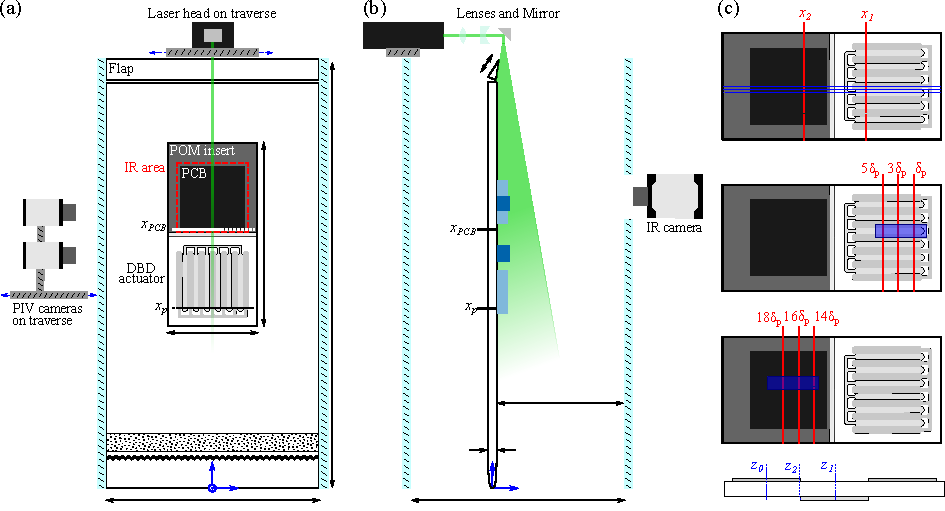
\includegraphics[width = 0.99\textwidth]{figures/methodology/setup_all_rebut.pdf}
    \caption{Schematic of the experimental setup and measuring stations. The coordinate system origin is set at the leading edge. Actuation begins at $x_p = 421\mathrm{mm}$. (a) Front view; the measurement area of infrared thermography is indicated \lcap{--}{red}. (b) Side view.; the field of view of the planar-PIV \sy{blue2}{rec} and stereo-PIV \sy{blue6}{rec} measurements are highlighted. (c) From top to bottom: streamwise \lcap{--}{red} and spanwise \lcap{--}{blue} station in planar-PIV measurements ($x_1=530\mathrm{mm}$, $x_2=675\mathrm{mm}$); region of measurement \sy{blue}{rec} and selected $\hat{x}$-planes \lcap{--}{red} for stereo-PIV; spanwise stations \lcap{--}{blue} over the cross-section of a couple of electrodes ($z_2=-6.5\mathrm{mm}$, $z_1=-13\mathrm{mm}$, $z_0=0$).}
    \label{fig:setup}
\end{figure}

The turbulent boundary layer develops on a machined aluminum flat plate  (surface roughness $R_q: 0.05\mathrm{mm}$) of $1\mathrm{m}$ length and $20\mathrm{mm}$ thickness, spanning the entire width of the test section (see figure \ref{fig:setup}). Two parallel side walls ensure two-dimensional flow while two extra walls are mounted parallel to the flat plate model, closing the test section, thus approximating zero-pressure-gradient conditions on the model. To measure the pressure distribution, the flat plate is equipped with $81$ static pressure taps spaced by $15\mathrm{mm}$ in the streamwise direction. The plate is equipped with plasma actuators and with a convective heat transfer sensor, both flush-mounted by means of polyoxymethylene (POM) inserts.

The flat plate leading edge follows a modified super-ellipse \citep{Lin1992LEeffect} to reduce curvature discontinuities. The leading edge stagnation point is controlled by a $50\mathrm{mm}$ long adjustable trailing-edge flap, deflected by approximately $15^\circ$. The boundary layer is tripped close to the leading edge with zig-zag turbulators of $1.9\mathrm{mm}$ height located at $x = 0.06\mathrm{m}$. The turbulators are followed by a $50\mathrm{mm}$ wide strip of silicon carbide grit with a characteristic height of $1\mathrm{mm}$, guaranteeing a random distribution of surface irregularities to eliminate coherent structures from the zig-zag turbulator. Care is taken to ensure that the turbulent boundary layer at the measurement locations is not affected by tripping effects \citep{sanmiguel2017diagnostic}.

%-----------------------------------------------------------------------------
%%%%%%%%%%%%%%%%%%%%%%%%%%%% PLASMA ACTUATOR  %%%%%%%%%%%%%%%%%%%%%%%%%%%%%%%%
\subsection{DBD-Plasma Actuator configuration \label{ss:PlasmaActuator}}
%-----------------------------------------------------------------------------
The DBD-plasma actuator layout is shown in figure~\ref{fig:3D_PA_detail}. The actuator assembly consists of a repeated pattern of 6 linear bi-directional actuators with spanwise wavelength $\lambda = 26 \mathrm{mm}$ and streamwise length $L = 128 \mathrm{mm}$. The electrodes are aligned parallel to the oncoming flow. Each actuator makes use of two air-exposed electrodes and one covered electrode. Neighbouring actuators make use of common exposed electrodes as well, which yields the formation of plasma on both sides of each exposed electrode. As shown later, the resulting body force distribution produces a sequence of opposing wall jets tangent to the surface in the spanwise direction which interacts with the external flow, eventually generating pairs of counter-rotating streamwise vortices with size $O(\lambda/2)$. This plasma-induced motion enhances the cross-stream mixing of momentum within the TBL, serving as the basic mechanism for flow control. The electrode array shown in figure~\ref{fig:3D_PA_detail} differs from the single streamwise-oriented DBD-actuator investigated by \citet{jukes2013plasmaVG}; however, it is very similar, both in shape and characteristics, to the Plasma Streamwise Vortex Generator (PSGV) proposed by \citet{Wicks2015} to generate streamwise vorticity within a TBL and to the Configurations A and B proposed by \citet{cheng_wong_hussain_schroder_zhou_2021} to reduce skin-friction drag within a TBL over a flat plate. The readers are referred to \citet{Kelley2016} for further insights on the design and scaling of plasma vortex generators.
%-------------------------------------------------------------------------------
\begin{figure}[t]
    \centering
    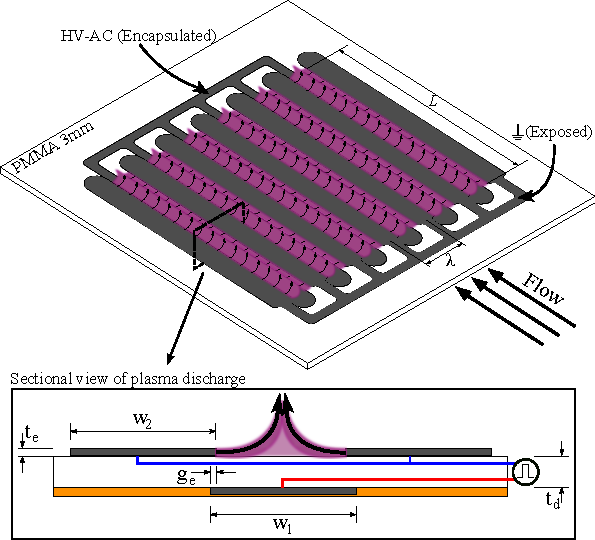
\includegraphics[width = 0.65\linewidth]{figures/methodology/3D_PA_detail_v3.pdf}
    \caption{DBD-plasma actuator array schematic. Geometrical parameters are defined in the detailed view of the DBD-plasma actuator section. The interspersed array of encapsulated and exposed electrodes \sy{electrode}{rec} is depicted. The plasma glow discharge is outlined \sy{plasma}{rec} and the polyamide insulation is highlighted \sy{kapton}{rec} for clearness.}  \label{fig:3D_PA_detail}
\end{figure}
%-------------------------------------------------------------------------------

The electrodes are manufactured using deposition of conductive silver particles in a 2-butanone solution, allowing for thin, smooth electrodes of negligible roughness $(< 10 \upmu \mathrm{m})$. Unlike previous studies using a thin dielectric barrier for streamwise-oriented actuators in laminar boundary layers \citep{Jukes2012,jukes2013plasmaVG}, control of separation in airfoils \citep{jukes2013nacaVG}, promotion of spanwise-travelling waves within a TBL \citep{Whalley2014} or streamwise-vortex generators \citep{cheng_wong_hussain_schroder_zhou_2021}, this study follows the recommendations from the work by \citet{thomas2009dbdopt}, who demonstrated a better than an order-of-magnitude increase in the plasma-induced body force produced by actuators for thicker dielectric barriers. Consequently, the arrays of exposed and covered electrodes are separated by a dielectric material (PMMA) of $3 \mathrm{mm}$ thickness (similar to the quartz dielectric used by \citet{Wicks2015} and $\approx 13$ times thicker than in \citet{Jukes2012,jukes2013plasmaVG, Whalley2014,cheng_wong_hussain_schroder_zhou_2021}. Degradation of plasma actuators, when subjected to high voltage for a long time, has been recently reported by \citet{cheng_wong_hussain_schroder_zhou_2021}. The choice of the dielectric material does not only affect the intensity of the actuation but also the robustness of the device as well as the heat generation. The plasma actuator hereby described is capable of reliably operating for long periods without loss of effectiveness, allowing the use of a single actuator array for the whole experimental campaign. Moreover, despite the fact that thicker dielectrics tend to promote higher gas heating \citep{Rodrigues2018b}, it was ensured that the actuator does not provide sufficient thermal footprint that could affect the convective heat transfer measurements.

The actuator assembly is installed on an insert manufactured with the same dielectric material. The assembly allows for a flush-mounted design in the aluminium flat plate, largely minimising surface protrusions or irregularities that can affect the developing flow. Furthermore, polyimide (Kapton) tape is used to insulate the covered electrode and the edges of the actuator plate in order to avoid spurious plasma discharges. Details on the geometrical and material properties of the plasma actuator are listed in Table \ref{tab:actuatorparam}. The actuator array is driven by a TREK 20/20C HS high-voltage amplifier, connected to the covered electrodes, while the air-exposed electrodes are kept at ground potential. A dielectric barrier discharge of weakly-ionised air is achieved using a sinusoidal voltage signal at a frequency of $2\mathrm{kHz}$. The choice of carrier frequency is made as a compromise between power delivery limitations of the TREK amplifier and sufficient separation of hydrodynamic scales. Indeed, for the present study, the carrier frequency, scaled in wall units $f_d^+ \approx 0.1$ is significantly larger than the inverse of the convective time unit of the reference TBL, $U_\infty^+/Re_\tau$ $\approx 0.04$, %(Uinf/d99) / (utau^2/nu)
effectively rendering the action of the body force time-invariant.

%-----------------------------------------------------------------------------
\begin{table}[t]
\centering
\begin{tabular}{lll}
\toprule
% \multicolumn{2}{c}{Parameter} & Value \\ \midrule
$\lambda$ & Spanwise wavelength & 26.0 mm \\
$w_1$ & Exposed electrode width & 13.5 mm \\
$w_2$ & Covered electrode width & 13.5 mm \\
$t_d$ & Dielectric thickness & 3.0 mm \\
$g_e$ & Overlap between electrodes & $\sim$0.5 mm \\
$t_e$ & Electrode thickness & $<10$ $\mu$m \\
$l$ & Electrode length & 169.5 mm \\
$L$ & Effective plasma discharge length & 128 mm \\
$V_{pp}$ & Discharge voltage peak-to-peak & 10-20 kV \\
$f_d$ & Carrier frequency & 2 kHz \\ 
$P$ & Actuator power consumption & 150-300 W/m\\
\bottomrule
\end{tabular}
\caption{Geometrical, material and operation properties of the plasma actuator}\label{tab:actuatorparam}
\end{table}

%-----------------------------------------------------------------------------
%%%%%%%%%%%%%%%%%%%%%%%%%%%%%%%%%%% PIV  %%%%%%%%%%%%%%%%%%%%%%%%%%%%%%%%%%%%%
\subsection{Velocity measurements \label{ss:PIV}}
%-----------------------------------------------------------------------------
Velocity field measurements are performed using planar, two-component Particle Image Velocimetry (PIV) in several $x-y$ planes, i.e. parallel to the freestream and normal to the flat plate, as shown schematically in figure \ref{fig:setup}. Anticipating the strongly three-dimensional nature of the flow emerging from the actuation, additional stereoscopic PIV measurements are performed for selected actuation cases.

Seeding particles are produced by a SAFEX fog generator using a glycol-water solution with a mean droplet diameter of $1 \mu\mathrm{m}$ released in the wind tunnel circuit downstream of the test section. Illumination is provided by a dual cavity Nd:Yag Quantel Evergreen laser ($200\mathrm{mJ/pulse}$ at $15\mathrm{Hz}$) and a set of cylindrical and spherical lenses. The laser sheet thickness is approximately $1\mathrm{mm}$ for the planar-PIV cases and $3\mathrm{mm}$ for the stereo-PIV. 
Two LaVision Imager sCMOS CLHS cameras are used to image the flow. Three camera configurations are composed for planar (C1 and C2) and stereoscopic (C3) measurements, shown as shaded regions in figure \ref{fig:setup}. In configuration C1, the camera fields of view (FOV) are stitched in order to obtain a combined FOV of $190\times30 \mathrm{mm}^2$ at a magnification ratio of approximately 0.16, thus, allowing to obtain an overview of the global TBL development. In turn, C2 is used to obtain high-resolution measurements for extracting TBL statistics simultaneously at two different streamwise locations (see figure~\ref{fig:setup}), with each camera having a FOV of $45\times20 \mathrm{mm}^2$ and magnification ratio of 0.37. Finally, for the stereoscopic configuration C3, the FOV is $100\times20 \mathrm{mm}^2$ at a magnification of approximately 0.16. The total measurement area by PIV spans between $0.4m\leq x \leq 0.7m$, which covers the region of interest from the upstream edge of plasma actuation to the heat-flux sensor.
%------------------------------------------------------------------------------
\begin{table}
\centering
\begin{tabular}{lccc}
% \begin{tabular}{\tblwidth}{p{0.462\linewidth-2\tabcolsep} %@{}lcc@{}}
%                 >{\centering\arraybackslash}p{0.1793\linewidth-2\tabcolsep}
%                 >{\centering\arraybackslash}p{0.1793\linewidth-\tabcolsep}
%                 >{\centering\arraybackslash}p{0.1793\linewidth-2\tabcolsep}}
\toprule
\multicolumn{1}{l}{Parameter} & C1 & C2 & C3 \\ \midrule
Camera & \multicolumn{3}{c}{LaVision’s Imager sCMOS CLHS} \\
Sensor resolution & \multicolumn{3}{c}{2560$\times$2160 px$^2$} \\
Pixel pitch & \multicolumn{3}{c}{$6.5\mu$m} \\
PIV measurement type & Planar & Planar & Stereoscopic\\
Lens focal length [mm] & 60 & 105 & 60\\
Aperture $(f_{\#})$ & 5.6 & 5.6 & 8\\
Frame separation $(\Delta t)$ [$\mu$s] & $40$ & $20$ & $40$\\
Field of view (FOV) [mm$^2$] & $190 \times 30$ & $45 \times 20$ & $100 \times 20$\\
Digital resolution [px/mm] & 25.16 & 58.41 & 25.6 \\
Magnification factor & 0.16 & 0.37 & 0.16\\
Interrogation window [px$^2$] & 12$\times$12 & 12$\times$12 & 12$\times$12 \\
Overlap factor & 50\% & 50\% & 50\%\\
Vectors per velocity field & $791\times125$ & $450 \times 200$ & $434 \times 86$\\
Vector pitch [mm] & 0.24 & 0.10 & 0.23\\
\bottomrule
\end{tabular}
\caption{PIV parameters} \label{tab:PIVparam}
\end{table}
%------------------------------------------------------------------------------

For all camera configurations and actuation conditions, an ensemble of 1300 image pairs is acquired at a sampling frequency of 15Hz. Processing of the images is carried out using LaVision DaVis 10.1 software. A multi-pass %\citep{soria1996piv} 
cross-correlation algorithm \citep{Willert1991digitalpiv} with window deformation \citep{scarano2001iterativeimgdef} is applied to the sequence of images, with a final interrogation window size of $12\times12$ $\mathrm{pixels}^2$ and 50\% of overlap. Spurious vectors are discarded by applying a universal outlier detector \citep{westerweel2005outlier} and are replaced by interpolation based on adjacent data. A summary of the relevant PIV parameters is provided in table \ref{tab:PIVparam}. The convergence of first- and second-order statistics within a variation of 1.5\% has been confirmed for all cases.

In order to capture the three-dimensional flow features emerging from the operation of the plasma actuator array, the PIV system, including cameras and laser head, is mounted on an automated traverse system allowing precise scans in the spanwise direction. For the planar-PIV cases, five planes are measured: $z_0$, $z_1$, and $z_2$ as shown in figure~\ref{fig:setup}(c), as well as the symmetric planes of $z_1$ and $z_2$ with respect to $z_0$. A more refined scanning is performed for the stereo-PIV measurements, with a total of $18$ planes, equally spaced between $z=0$ and $z=25.5\;\mathrm{mm}$ as highlighted in figure~\ref{fig:setup}(c), allowing to obtain a fully reconstructed three-dimensional mean flow.

The experimental uncertainties associated with the PIV measurements are computed from the uncertainty estimation tool developed by \citet{Castellanos2021PIVuncertainty} for PIV/EPTV measurements. The uncertainty on the TBL parameter estimation is directly related to the averaging-window size in wall units. For the PIV configuration C2, the final interrogation window corresponds to a size of 12$l^*$ (where $l^* = \nu/u_\tau$ is the viscous length), which guarantees a high-resolution measurement for the estimation of TBL parameters. Hence, the uncertainty on the integral lengths $\delta^*$ and $\theta$ and the boundary-layer thickness $\delta$ is estimated to be below $\pm 2\%$. The uncertainty for the estimation of $U_\infty$ and $u_\tau$ is well below 1\% and the position of the wall is estimated with an error below $\Delta y^+ = \pm 5$. Note that the boundary-layer thickness $\delta$ is approximated in this study as $\delta \approx \delta_{99}$, such that $u(y=\delta_{99})=0.99U_\infty$.
% Remember that my WallUnit = ~2.8e-05 m

%------------------------------------------------------------------------------
%%%%%%%%%%%%%%%%%%%%%%%%%%%%%%%%%%%% IR %%%%%%%%%%%%%%%%%%%%%%%%%%%%%%%%%%%%%%%
\subsection{Infrared thermography measurements \label{ss:IR}}

Wall heat fluxes are assessed from convective heat transfer measurements, using infrared thermography. Measuring surface heat fluxes in thermo-fluid dynamics requires both heat-flux sensors and temperature transducers. In the present work, the temperature transducer is infrared thermography, in conjunction with a heated-thin-foil sensor, a common choice in heat transfer investigations \citep{astarita2012infrared}. The chosen heat-flux sensor in this study is fabricated as a Printed Circuit Board (PCB). A PCB similar to those used in \citet{torre2018HTF} is chemically bonded to a machined insert made of POM and flush-mounted into the flat plate. The PCB features a copper track with a thickness of $5\mathrm{\mu m}$, a pitch of 2 $\mathrm{mm}$ and a gap of 0.2 $\mathrm{mm}$. The heat-flux sensor can be considered isothermal across its thickness \citep{astarita2012infrared} since the Biot number ($\mathrm{Bi} = h t/k$, where $h$ is the convective heat transfer coefficient while $k$ and $t$ represent the foil thermal conductivity coefficient and thickness, respectively) is relatively small for the proposed problem $( \mathrm{Bi} \approx 0.003)$. The heat-flux sensor is placed at a distance of $0.6\mathrm{m}$ downstream of the leading edge, i.e. $50\mathrm{mm}$ downstream of the end of the plasma discharge. 

The PCB electrode has a nominal resistance of $25.5\Omega$, a circuit area $(A_{\mathrm{PCB}})$ of $150\times 150\mathrm{mm}^2$ and a thickness of $0.5\mathrm{mm}$. A constant heat-flux $q''_{j}$ is achieved using Joule heating enabled by a stabilised power supply connected to the PCB, which provides constant voltage $V$ and current $I$ ($q''_{j} = V I / A_{\mathrm{PCB}}$). The convective heat transfer coefficient distribution is expressed in non-dimensional form in terms of Stanton number ($St = h/(\rho_{\mathrm{air}}U_\infty C_{p_{\mathrm{air}}})$), where $\rho_{\mathrm{air}}$ is the air density, $U_\infty$ is the freestream velocity, $C_{p_{\mathrm{air}}}$ is the specific heat capacity of air. The computation of $h$ is performed through a steady-state energy balance, modeling the PCB as a heated-thin-foil sensor \citep{astarita2012infrared}, %------------------------------------------------------------------------------
\begin{equation}
	h = \frac{ q''_{j} - q''_{r} - q''_{k} }{ T_{w} - T_{aw} } ,
	\label{eq:heatedthinfoil}
\end{equation}
%------------------------------------------------------------------------------
where $T_{w}$ is the surface temperature of the PCB, $T_{aw}$ is the adiabatic wall temperature, $q''_{r}$ is the radiation heat flux and $q''_{k}$ is the tangential conduction heat flux through the PCB. Heat-flux losses due to natural convection on the rear side of the PCB are minimised with a $2 \mathrm{mm}$ air gap between the rear surface of the PCB and the POM-insert. These losses are estimated to be below 1\% of the convective heat transfer using correlations for natural convection into rectangular cavities \citep{bergman2011fundamentals}. Natural convection losses on the flow-facing side are neglected since $\mathrm{Gr/Re}^2<< 1$ ($\mathrm{Gr} = {g\beta_v(T_{w}-T_{aw}) L^3}/{\nu^2}$ is the Grashoff number, where $\beta_v$ is the volumetric thermal expansion coefficient and $g$ the acceleration of gravity). The radiative heat flux $q''_{r} = \sigma \varepsilon (T_w^4 - T_\infty^4)$ (where $\sigma$ is the Boltzmann constant and $\varepsilon$ is the emissivity of the PCB surface) is estimated under the assumption that the environment behaves like a blackbody with a temperature equal to that of the free stream $T_\infty$. Although the PCB copper tracks introduce an anisotropic thermal behaviour of the board, the PCB layout complies with the criteria proposed by \citet{torre2018HTF} with the tangential conduction losses through the plate being below 0.5\%, estimated according to $q''_{k} = kt \left( \frac{\partial^2T}{\partial x^2} + \frac{\partial^2T}{\partial y^2} \right)$.

The temperature measurements are performed with a CEDIP-SC7300 Titanium IR camera (320$\times$256 pixel MCT sensor and Noise Equivalent Temperature Difference (NETD)$<25\mathrm{mK}$.), capturing images at a frequency of $10\mathrm{Hz}$ with a spatial resolution of $1.6\mathrm{pixels/mm}$. To improve the accuracy of IR measurements the PCB is coated with a thin layer of high-emissivity paint ($\varepsilon = 0.95$). The value of the wall temperature ($T_w$) and the adiabatic temperature at the wall ($T_{aw}$) are computed from two different measurement runs: $T_{aw}$ is obtained as the ensemble average of 300 images acquired with $q_j''= 0$, henceforth referred to as \textit{cold} images; $T_w$ is the ensemble average of 300 images acquired with the PCB activated, referred to as \textit{hot} images. The experimental uncertainties associated with the measurements are determined through a Monte Carlo simulation \citep{minkina2009infrared}, assuming statistically uncorrelated errors and using the uncertainty values reported in table~\ref{tab:uncertainties}. The uncertainty on the local Stanton number is estimated to be $\pm 3.7\%$.

\begin{table}
\centering
\begin{tabular}{lll}
\toprule
Parameter & Uncertainty & Typical Value \\ \midrule
$T_w$ & 0.1 K & 297 [K]  \\
$T_{aw}$ & 0.2 K & 290 [K] \\
$T_\infty$ & 0.1 K & 292 [K] \\
$V$ & 0.2\% & 17 [V] \\
$I$ & 0.2\% & 0.65 [A] \\
$\varepsilon$ & 2\% & 0.95 \\
$A$ & 0.1\% & 225 [cm$^2$] \\
$C_{p_{\mathrm{air}}}$ & 1\% & 1006 [kJ/(kg K)] \\
$\rho_{\mathrm{air}}$ & 1\% & 1.224 [kg/m$^3$] \\
$U_\infty$ & 1\% & 11.8 m/s \\
$q''_k$ & 10\% & 0.6 [W/m$^2$] \\ 
\bottomrule
\end{tabular}
\caption{Uncertainty Analysis on Stanton number calculation} \label{tab:uncertainties}
\end{table}
%------------------------------------------------------------------------------
%%%%%%%%%%%%%%%%%%%%%%%%%%%%%%%%%%%% Plasma characterization %%%%%%%%%%%%%%%%%%%%%%%%%%%%%%%%%%%%%%%
\subsection{Momentum coefficient at quiescent conditions} \label{ss:plasma_char}
%
\begin{figure}
    \centering
    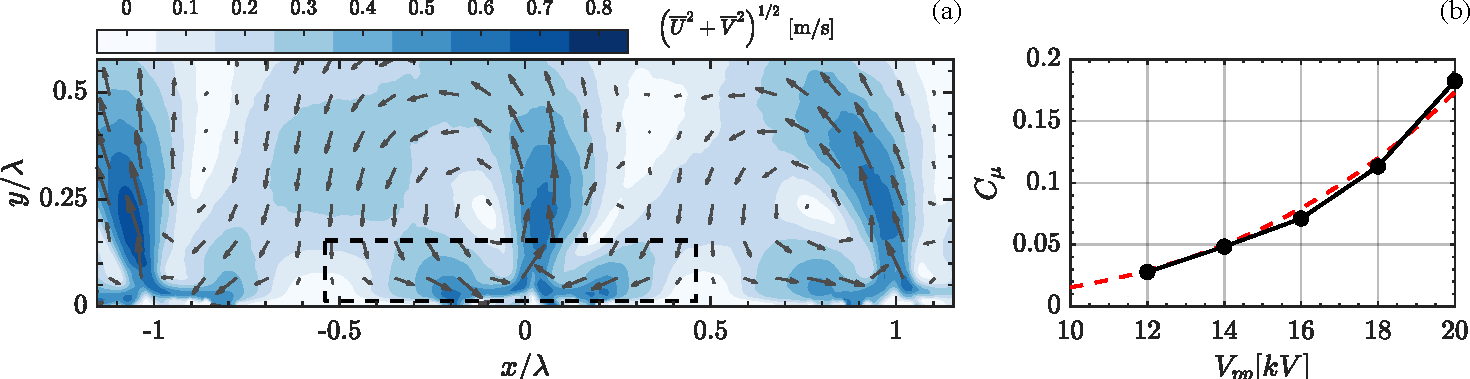
\includegraphics[width = 0.99\textwidth]{figures/methodology/plasmachar_rebut.pdf}
    \caption{Plasma characterisation. (a) Contour of the induced plasma flow velocity magnitude. The control volume for the momentum balance is highlighted \lcap{--}{black}. (b) Momentum coefficient as a function of the discharge voltage \sy{black}{o*} and experimental fit for empirical relation $C_\mu \propto V_{pp}^{7/2}$ \lcap{--}{red}} %cmu = [0 0.0153315757803183,0.0277902175268809,0.0483544971252209,0.0711091393955022,0.113346894209305,0.182458139582648];
    \label{fig:plasma_char}
\end{figure}
%
The body force produced by a DBD-plasma actuator can be directly identified as a source term in the Navier-Stokes equations, enabling the active addition of momentum to the fluid. This can be expressed in terms of momentum coefficient ($C_\mu$) \citep{Amitay2001Cmu},
\begin{equation} \label{eq:Cmu}
    C_\mu = \frac{\mathbf{\overline{I}}}{1/2\rho_\infty U_\infty^2 L}.
\end{equation}
The time-averaged momentum per unit length, $\mathbf{\overline{I}}$, is normalised by the fluid density, $\rho_\infty$, the square of the free stream velocity, $U_\infty$, and the length of the plasma actuator, $L$. In turn, $\mathbf{\overline{I}}$ is calculated as described by \citet{kotsonis2015control}, through the application of the momentum balance equation,
\begin{equation}
    \mathbf{\overline{I}} = \oint_S \rho_\infty \mathbf{\overline{u}} \left( \mathbf{\overline{u}} \cdot \mathbf{\hat{n}}  \right) \,dS,
\end{equation}
on the appropriate control volume, $S$, assuming negligible pressure contribution. Furthermore, for the conditions considered in this work, electrodynamic scales can be considered sufficiently separated from hydrodynamic scales. Consequently, the produced momentum is assumed independent of the freestream velocity \citep{Pereira2014external}, allowing quiescent conditions to be chosen for characterisation purposes. Measurements of the velocity fields at different voltage amplitudes and for continuous operation of the actuator at 2kHz carrier frequency are performed by planar-PIV in a setup dedicated to momentum coefficient quantification. The latter consists of a chamber with optical access, ensuring quiescent conditions, wherein the actuator array is placed. The chamber is filled with seeding generated by dielectric paraffin oil. Images are captured at the midspan of the electrodes $(L/2)$ over a field of view of $65\times21\mathrm{mm}^2$ and are processed to obtain velocity fields of $351\times116$ vectors at a vector pitch of 0.18mm in both directions.

A representative, time-averaged flow field of the actuator at $V_{pp} = 20\mathrm{kV}$ along with the estimated momentum coefficient for a range of peak-to-peak voltages are shown in figure~\ref{fig:plasma_char}. The actuator layout ensures a spanwise periodicity of the mean flow pattern, where the opposing jets collide and are redirected in the wall-normal direction, causing a distinct wall-normal jet whose maximum velocity is approximately 0.7 m/s at the highest discharge voltage. Since the control volume used for estimating the momentum coefficient contains the two opposing streamwise jets, the largest contribution in force originates from the momentum exchange along the $y$-direction ($C_{\mu} \approx C_{\mu_y}$), while in the $z$-direction momentum exchange is approximately zero. Characterisation is performed for a range of discharge voltages from $10\mathrm{kV_{pp}}$ to $20\mathrm{kV_{pp}}$, however, measurements at $10\mathrm{kV_{pp}}$ are not reliable. At these conditions, the induced jet velocities are very low, hence, the seeding cannot be adequately distributed in the vicinity of the actuator, causing gaps in regions relevant for estimation of the momentum coefficient. Nonetheless, through the remainder of discharge voltages, it is evident that the momentum coefficient follows the well established $7/2$th power-law, firstly proposed in \citet{Enloe2004} and later reported in numerous experiments \citep{thomas2009dbdopt,Mertz2011}.% and corke2009sdbd.
Although the $\mathrm{Re}$ number of the herein considered TBL is comparable to the one in \citet{cheng_wong_hussain_schroder_zhou_2021}, the present study is performed at a much higher freestream velocity, hence, there are higher requirements of momentum coefficient from the actuator.

%%%%%%%%%%%%%%%%%%%%%%%%%%%%%%%%%%%%%%%%%%%%%%%%%%%%%%%%%%%%%%%%%%%%%%%%%%%%%%
%%%%%%%%%%%%%%%%%%%%%%%% stereo-PIV %%%%%%%%%%%%%%%%%%%%%%%%%%%%%%%%%%%%%%%%%
%%%%%%%%%%%%%%%%%%%%%%%%%%%%%%%%%%%%%%%%%%%%%%%%%%%%%%%%%%%%%%%%%%%%%%%%%%%%%%
\section{Time-averaged flow field}\label{s:stereo}
%
\begin{figure}
         \centering
         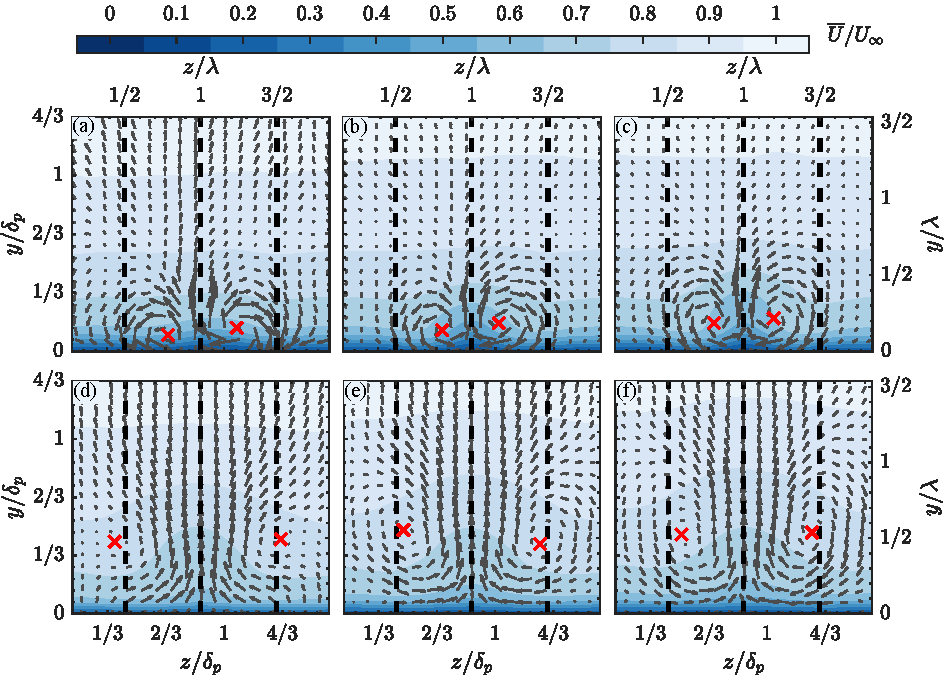
\includegraphics[width=0.99\textwidth]{figures/results/stereo/stereo_rebut.pdf}
         \caption{Evolution of plasma-induced large structures for the strongest actuation case ($V_{pp} = 20 \mathrm{kV}$, $C_\mu = 0.1825$) in the $y-z$ plane at $\hat{x} = \delta_p,~3\delta_p,~5\delta_p$ over the actuator (a-c) and $\hat{x} = 14\delta_p,~16\delta_p,~18\delta_p$ downstream of the actuation (d - f). The contour depicts the streamwise velocity distribution at each plane. The quiver represents the in-plane flow motion ($\overline{V}$,$\overline{W}$). The center of the vortex core based on $Q$-criterion is highlighted \sy{red}{x}.  From left to right, spanwise stations $z_2'$, $z_1$ and $z_2$ are highlighted \lcap{--}{black} (see figure~\ref{fig:setup}).} \label{fig:Ucont_quiver}
\end{figure}
%
As established in the previous sections, the actuator array is designed to produce strong spanwise modulations in the boundary layer, via tangential and opposing momentum addition.

The topology of the plasma-induced flow for the strongest actuation case (i.e., $V_{pp} = 20\mathrm{kV}$) is depicted in figure~\ref{fig:Ucont_quiver} for the selected locations over the flat-plate model as shown in figure~\ref{fig:setup}(c). The streamwise coordinate is defined as $\hat{x}=x-x_p$, where $x_p = 421\mathrm{mm}$ is the location of the upstream edge of the plasma discharge (being the origin located at the leading edge of the flat plate). The streamwise coordinate is normalised with the boundary-layer thickness at $x_p$, $\delta_p$, while the spanwise coordinates with the actuator wavelength $\lambda$. Figure~\ref{fig:Ucont_quiver} depicts the average streamwise velocity $\overline{U}$ on the $y-z$ plane at $\hat{x} = \delta_p,~3\delta_p,$ and $~5\delta_p$ along with a superimposed vector plot of the corresponding $\overline{V}$ and $\overline{W}$ velocity components. On the most upstream location of actuation ($\hat{x} = 0$), the fluid ejected laterally by the discharge is replenished by entertainment from above the exposed electrodes. This generates a vortical motion in the streamwise direction. The coalescence of the plasma-induced circulation with the main stream leads to twisting and folding of the spanwise vorticity at the tip of each plasma actuator. The latter causes streamwise-vortices to roll up and evolve as a partially developing starting vortex. The general evolution of this structure is similar to the observations of \citet{jukes2013plasmaVG} for a laminar boundary layer. Note, however, that the mechanism of the streamwise vortex formation differs from the creation of a starting vortex at quiescent air conditions, which is generated by the entrainment of fluid directly above the plasma region as reported by \citet{Whalley2010DBDvortex,Whalley2012startingV}. At $\hat{x} = \delta_p$, the streamwise vortices are already developed and begin to depart from the wall; their core is located at approximately $y\approx \delta_p/10$. The counter-rotating, streamwise vortices collide at $z_1$ leading to a strong upwash motion while the suction effect above the exposed electrodes keeps bringing air towards the wall at $z_2$. While the streamwise vortices develop in a region which coincides with the actuator, they are continuously strengthened, being displaced out of the wall by mutual induction \citep{Jukes2012}. The intensity of the vortices is mainly raised by the continuous momentum injection promoted by the DBD-actuator, although their interaction may exacerbate such effect \citep{Logdberg2009}. According to \citet{Pauley1988,Pauley1994}, the image vortices \citep{Ersoy1985} cause the pair of counter-rotating vortices with common upflow to move towards each other until they come to close proximity where the effect of their images cancel out. Subsequently, the vortices convect away from the wall.

The ejection of fluid normal and away from the wall at the plain of symmetry between counter-rotating vortices has been recently exploited in \citet{cheng_wong_hussain_schroder_zhou_2021} to control the turbulence regeneration mechanism within a TBL with a similar plasma-actuator array. Additionally, the pair of counter-rotating, streamwise vortices is confined in the space between two consecutive, opposing, exposed electrodes, i.e. $1/2<z/\lambda<3/2$ according to figure~\ref{fig:Ucont_quiver}, suggesting vortex stationarity.
The stationarity of the vortices in the present study has been confirmed with Proper Orthogonal Decomposition (POD) \citep{Lumley1967} during preliminary assessments on both planar- and stereo-PIV data, confirming the absence of any long-wavelength flapping modes. 

While the effect of the actuator is evident in streamwise locations where the discharge is active, it is striking to monitor the evolution of the flow field further downstream, up to $x_p\approx 20\delta_p$ (figure \ref{fig:Ucont_quiver} d-f). Although these locations are well downstream of the end of the discharge region, the effect of the actuation is still persisting. The induced structures are strong enough to divert the flow even $18\delta_p$ downstream of the plasma onset. At this streamwise location, the perturbation starts affecting also the outer region of the boundary layer via a lift-up action of the vortices towards the outer region. The region with significant spanwise velocity induced by the plasma discharge is also characterised by a low-speed streamwise velocity and is located in the gap between adjacent, opposing exposed electrodes. Nevertheless, an important consequence of the vortices interacting is their weakening along the downstream direction due to their continuous planar re-connection via cross-diffusion \citep{Hussain2011,Yao2020}. The vortices progressively expand in the spanwise direction and lose strength, in agreement with \citet{Wicks2015}. Nonetheless, the mutual interaction between the pair of vortices yields a strong wall-normal velocity that clearly persists at $\hat{x} = 14\delta_p$ and which is progressively expanded over a wider area in the spanwise direction.

\citet{Wicks2015} demonstrated that the streamwise vorticity generation is proportional to the actuator length $L$ for fixed $U_\infty$, and that the optimum inter-electrode spacing $\lambda$ is decoupled from the incoming boundary layer, being solely driven by the physics of plasma discharge. In agreement with these observations, the proposed DBD-actuator promotes strong streamwise vortices with a reminiscent and persistent effect downstream of the actuation. Moreover, the spanwise wavelength $\lambda$ is adequate to ensure the local confinement of the streamwise vortices along the electrodes.

The observed topology of the plasma-induced flow field is in agreement with the recent findings reported by \citet{cheng_wong_hussain_schroder_zhou_2021}, in which the authors conclude, from smoke-wire flow visualisation, that upon activation of control, the TBL streaks tend to merge and stabilise due to the effect of the large-scale streamwise vortices. Comparable velocity deficit has also been observed in the boundary layer with streamwise vortices induced by sub-boundary-layer vortex generators \citep{Sandborn1981}. On the other hand, high-speed fluid is trapped between the low-speed fluid ribbons due to the downwash of the streamwise vortices.

The injected momentum by the plasma actuation lifts up the near-wall flow, which eventually gives rise to streamwise vorticity, in a manner analogous to conventional vortex generators. A body force perpendicular to the freestream induces a spanwise mean velocity gradient $\partial\bar{U}/\partial z$, yielding wall-normal mean vorticity $\overline{\omega}_y$. The combination of the plasma-induced flow with the main stream causes vorticity reorientation towards the streamwise direction mainly due to the mean strain rate $\partial\bar{U}/\partial y$. Likewise, the spanwise mean vorticity in the boundary layer $\overline{\omega}_z\approx\partial\bar{U}/\partial y$ is also reoriented into the streamwise direction by the actuator-induced spanwise mean velocity gradient $\partial\bar{U}/\partial z$. This vorticity redistribution mechanism is responsible for the generation of streamwise vortices. This interaction between the boundary layer and plasma-induced body force significantly augments the production of $\overline{\omega}_x$. Since the actuator body force scales with $V_{pp}^{3.5}$ (as demonstrated in \S\ref{ss:plasma_char}), it can be concluded that the actuator-induced $\overline{\omega}_x$, and hence the intensity of the vortices, also scales with the magnitude of the body force $|F_B|$ \citep{Wicks2015}.

%%%%%%%%%%%%%%%%%%%%%%%%%%%%%%%%%%%%%%%%%%%%%%%%%%%%%%%%%%%%%%%%%%%%%%%%%%%%%%
%%%%%%%%%%%%%%%%%%%%%%%%%%%%%%% TBL  %%%%%%%%%%%%%%%%%%%%%%%%%%%%%%%%%%%%%%
%%%%%%%%%%%%%%%%%%%%%%%%%%%%%%%%%%%%%%%%%%%%%%%%%%%%%%%%%%%%%%%%%%%%%%%%%%%%%%
\section{Turbulent Boundary Layer analysis } \label{s:TBLanalysis}
%
The effect of plasma forcing on the statistical description of the boundary layer at different values of the introduced momentum coefficient is evaluated, based on the high-resolution planar-PIV measurements. The experimental study is executed for the same DBD-plasma actuator layout under a range of discharge voltages to assess the effect of the actuation depending on its relative intensity with respect to the freestream. Considering the power law governing the forcing intensity to voltage, the cases are evaluated in terms of momentum coefficient although the discharge voltage is used as the label for clearness in the figures. For conciseness, the TBL analysis is only shown for the representative cases $V_{pp} = 0,10,18,20\mathrm{kV}$, where $V_{pp}=0\mathrm{kV}$ corresponds to the reference boundary layer without actuation.

The TBL statistics and profiles are obtained at selected streamwise and spanwise locations over the flat-plate model as depicted in figure~\ref{fig:setup}(c). For the subsequent analysis, two streamwise stations are selected: $x_1 = 0.53\mathrm{m} = {x}_p + 8\delta_p$; and $x_2 = 0.65\mathrm{m} = {x}_p + 16\delta_p$. The former allows monitoring of the effect of the plasma actuation on the TBL at the actuator region, while the latter focuses on the wake, far downstream of actuation. Similarly, the selected spanwise stations (see figure~\ref{fig:setup}(c)) are: $z_1 = -\lambda/2 =-13\mathrm{mm}$, coinciding with the intersection of the two opposing plasma discharges; and $z_2 = -\lambda/4 = -6.5\mathrm{mm}$, placed 0.25mm towards the suction side of the exposed electrode. 

The results are presented in inner unit scaling, with the corresponding normalisation with the friction velocity $u_\tau$ and the kinematic viscosity $\nu$. The value of $\nu$ is adjusted for each independent profile based on Sutherland's law \citep{Sutherland1893law}, using the ambient pressure and temperature measurements of the incoming flow. The value of $u_\tau$ for the non-actuated boundary layer is obtained by fitting the composite profile proposed by \citet{chauhan2009}. Note that fitting methods, as herein utilised, cannot be used for manipulated boundary layers. The value of $u_{\tau}$ for the non-actuated configuration is, therefore, used as the reference for both the non-actuated and the plasma-actuated flow. The considered normalisation ensures that all profiles collapse in the outer region. The normalisation of the TBL profiles with the local friction velocity (not available from the experimental measurements), which is considerably altered by the action of the plasma-induced streamwise vortices, would imply a shift of the profiles. This approach is followed in \citet{cheng_wong_hussain_schroder_zhou_2021}, in which hot-wire data was available, and hence, it becomes difficult to compare results.

%-----------------------------------------------------------------------------
%%%%%%%%%%%%%%%%%%%%%%%%%%%%%%%%%%%% TBL %%%%%%%%%%%%%%%%%%%%%%%%%%%%%%%%%%%%%
\subsection{Characterisation of the reference TBL \label{ss:refTBL}}
%-----------------------------------------------------------------------------
Characterisation of the reference turbulent boundary layer begins by assessing the streamwise pressure gradient using data from pressure taps. A weak favourable pressure gradient along the flat plate is identified with pressure coefficient values of $-0.02 \leq C_\mathrm{p} \leq 0.02$ in the region of interest.
The absolute value of the Clauser pressure-gradient parameter computed for the reference TBL is below 0.003, which is considered to be sufficiently low for a representative zero-pressure-gradient (ZPG) condition with minimal effect on the statistics as demonstrated in \citet{guemes2019APG}.

For the determination of mean wall-shear stress and the corresponding friction velocity as well as for boundary-layer parameter estimation, high-resolution PIV measurements are employed (described in \S\ref{ss:PIV} as configuration C2). In this work, the composite profile by \citet{chauhan2009} is used to infer the actual wall-position and the value of the friction velocity, by fitting the experimental data up to $y^+ = 30$. The robustness of this method has been well established, provided that near-wall measurements are available \citep{orlu2010wallpos,rodriguez2015skinfric,vinuesa2016nagib}. To this end, planar, high-resolution PIV measurements allowed to obtain a sufficiently large number of points within the buffer region to correct for the absolute wall position and determine the friction velocity without relying on log-law constants.

Care is taken to ensure a well-behaved TBL in the region of interest, from $x_p$ to the downstream edge of the PCB. The mean streamwise velocity profile, $\overline{U}^+$, measured at the downstream edge of the plasma actuator ($x=x_p + L$ , $z = 0$) is shown in figure~\ref{fig:TBLref}, fitted on the composite profile by \citet{chauhan2009}. The TBL profile agrees well with \citet{jimenez2010} DNS data. The method proposed by \citet{sanmiguel2017diagnostic}, based on the diagnostic plot \citep{alfredsson2011diagnostic}, is employed to assess the convergence towards a well-behaved ZPG TBL. The diagnostic plot parameters are attached in table~\ref{tab:diagnostic}, concluding the agreement with DNS data and with the empirical correlations of the method. In addition, complementary boundary-layer parameters of the TBL without actuation are reported in table \ref{tab:TBLparams}.

\begin{figure}
    \centering
    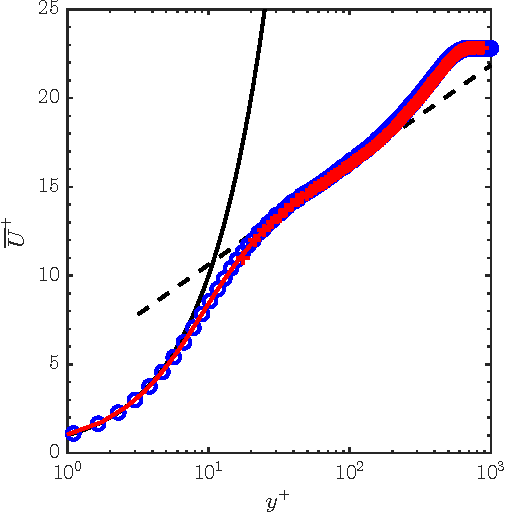
\includegraphics[width = 0.7\linewidth]{figures/methodology/TBLref.pdf}
    \caption{Profiles of the reference TBL at the downstream edge of the plasma actuator ($x=x_p+L$). PIV experimental data \sy{red}{+} is depicted together with its fit based on \citet{chauhan2009} \lcap{-}{red} and compared against DNS data from \citet{jimenez2010} \sy{blue}{o}. The viscous sublayer $U^+ = y^+$ \lcap{-}{black}, and the logarithmic law $U^+=\frac{1}{0.41} \mathrm{ln}y^+ + 5.0$ \lcap{--}{black} are included for reference.}
    \label{fig:TBLref}
\end{figure}
%----------------------------------------------------------------------------
\begin{table}
\centering
\begin{tabular}{llcc}
\toprule
Case & $Re_\theta$ & $\alpha$ & $\beta$ \\ \midrule
Reference TBL & 1596 & 0.28 ($-4.3\%$) & 0.25 ($-4.1\%$) \\
\citet{jimenez2010} & 1592 & 0.30 ($+4.1\%$) & 0.27 ($+2.5\%$) \\
\bottomrule
\end{tabular}
\caption{Diagnostic plot parameters of the reference TBL depicted in figure~\ref{fig:TBLref} and the DNS data from \citet{jimenez2010}. Error with respect to the method by \citet{sanmiguel2017diagnostic} between brackets.}\label{tab:diagnostic}
\end{table}
%----------------------------------------------------------------------------

%------------------------------------------------------------------------------
%%%%%%%%%%%%%%%%%%%%%%%%%%%%% mean-actuated TBL %%%%%%%%%%%%%%%%%%%%%%%%%%%%%
\subsection{Plasma forcing effect on the mean flow field \label{ss:meanTBL}}
%------------------------------------------------------------------------------
The $\overline{U}^+$ and $\overline{V}^+$ mean velocity profiles are shown in figure~\ref{fig:UmVmprofile} for the selected $x$ and $z$ locations. It should be noted that the results at the plane of symmetry ($z=0$) are not evaluated in this analysis as in that region the effect of the plasma actuation is negligible. Instead, the plasma forcing action is localised in the vicinity of the discharge edge of the electrode ($z_2$) and in the stagnation area where the two opposing jets collide ($z_1$). 

For the weakest forcing ($C_\mu = 0.0153$, i.e.  $V_{pp}=10\mathrm{kV}$), minimal flow distortion is observed, restricted in the near-wall region ($y^+<50$). Nevertheless, the effect of actuation intensifies with increasing momentum coefficient, while the mean flow deformation identified throughout the TBL extends from the wall to the outer region. The plasma actuator imparts two main changes to the mean flow: a suction effect at the edge of the exposed electrode, extracting fluid from the upper region of the boundary layer towards the wall and hence considerably modifying the inner region of the boundary layer, as shown in figures~\ref{fig:UmVmprofile}(b,f); and a momentum injection perpendicular to the main stream directly induced by the plasma actuator, distorting the TBL profile from the viscous sublayer up to $y^+\approx 400$ as shown in figures~\ref{fig:UmVmprofile}(a,e). These two contributions, although induced by the same actuation, promote substantially disparate effects on the TBL. Similar results have been recently reported by \citet{cheng_wong_hussain_schroder_zhou_2021}. It is to be noted, however, that the aforementioned study reports a non-monotonic increase of the actuation effectiveness with momentum injection (i.e discharge voltage). The authors claim that there exists an optimum discharge voltage for which drag reduction is maximized while further increasing the momentum injection would be detrimental since the induced vortices grow rapidly, causing an increase in vortex-induced shear stress. The present study shows a monotonic increase of the actuation effectiveness with momentum coefficient; however, discrepancies may be due to the considered discharge voltages and freestream velocity, which are up to 4 and 5 times higher in the present study, respectively. 

\begin{figure}[h!] % TBL profiles
    \centering
    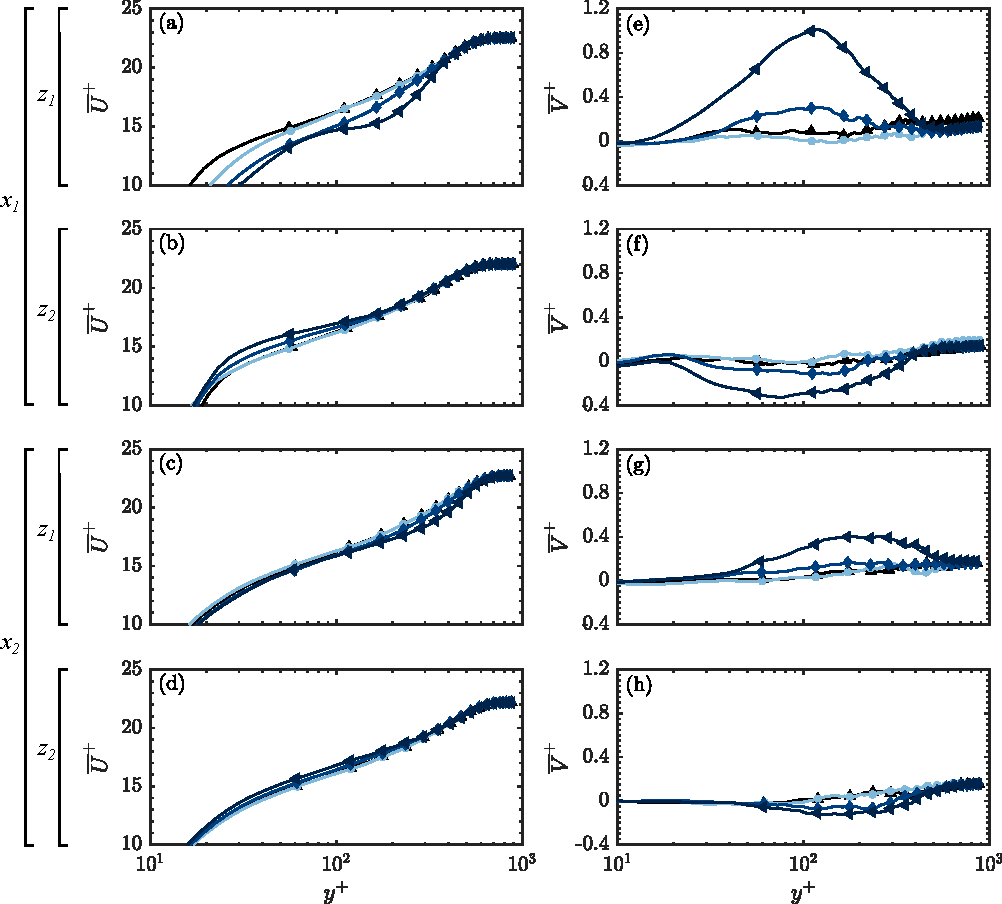
\includegraphics[width = 0.99\textwidth]{figures/results/TBL/U_V_profilesv3.pdf}
    \caption{Inner-scaled mean velocity profiles at selected stations according to figure~\ref{fig:setup}. Streamwise and wall-normal velocity profiles are depicted in the left column (a-d) and right column (e-h) respectively, for selected discharge voltages $V_{pp}=$ (and momentum coefficient $C_\mu = $) 0 \sy{black}{t*}, 10 (0.0153) \sy{blue2}{o*}, 18 (0.1133) \sy{blue6}{d*}, 20 (0.1825) \sy{blue7}{lt*}.}
    \label{fig:UmVmprofile}
\end{figure}%

From the $\overline{V}^+$ profiles, it is evident that the main perturbation on the reference flow manifests at $z_1$ for the strongest forcing case ($c_{\mu} = 0.1825$), characterised by a peak of positive wall-normal velocity at $y^+\approx 100$ in the vicinity of the actuator. This peak is a direct consequence of the opposing plasma-induced jets interacting, which eventually lift up from the wall causing a strong wall-normal motion. This effect is in agreement with the $\overline{U}^+$ profiles, in which a clear velocity deficit is induced by the forcing close to the wall.
Although the abrupt change in wall-normal velocity is only visible for the strongest forcing cases, the deficit in streamwise velocity is evident even for the weakest actuation. It can be conjectured that the changes are, therefore, limited to the inner part of the boundary layer, while for stronger actuation a larger-scale effect is observed, with the penetration of the perturbation towards the outer layer.

Downstream of the actuator ($x_2$), the dissipation of the induced motion becomes clear; however, a significant deficit of $\overline{U}^+$ is identified in figure~\ref{fig:UmVmprofile}(c), with displacements visible up to the outer region of the TBL. Analogously, the $\overline{V}^+$ peak is also progressively displaced away from the wall with a considerable reduction in magnitude (see figure~\ref{fig:UmVmprofile}g). It is evident that, while the injection of momentum in the wall-normal direction rapidly dissipates, the modification of the inner region is persistent.

The action of the plasma forcing in the suction side $z_2$
is characterised by a negative wall-normal velocity component above the wall as shown in figure~\ref{fig:UmVmprofile}(f). The flow accelerates in the streamwise direction, causing a raise in $\overline{U}^+$ slightly above the wall in the vicinity of the actuator (see figure~\ref{fig:UmVmprofile}b). The local pressure reduction, as a consequence of the suction, is responsible for the acceleration of the fluid. Both effects are strong enough to propagate downstream while displacing the local disturbances further from the wall as depicted in figures~\ref{fig:UmVmprofile}(d)~and~\ref{fig:UmVmprofile}(h).

Following the previous discussion on the effect of plasma actuation on the TBL, an analysis is performed on the evolution of $\delta$, $\delta^*$, and $\theta$. These TBL parameters for each of the evaluated cases are provided in table~\ref{tab:TBLparams}. The non-actuated TBL, highlighted in bold, is characterised by a shape factor of $H=1.46$, and a Reynolds number based on friction velocity $Re_\tau=\delta u\tau/\nu$ ranging from $582$ to $644$ between $x_1$ and $x_2$. The effect of the actuation is better understood from the variation of the parameters with respect to the non-actuated case that is within brackets. The variation of boundary-layer parameters is visualised in figure~\ref{fig:TBLstats_xz} along the streamwise and spanwise direction. The results depicted in figure~\ref{fig:TBLstats_xz}(a-c) and figure~\ref{fig:TBLstats_xz}(d-f) are computed from the stereo-PIV (C3) and planar-PIV (C1) measurements, respectively. Despite the lower resolution provided by measurement configurations C1 and C3, these results provide an overall insight of the TBL parameters distribution, with values in accordance to those reported in table~\ref{tab:TBLparams} computed from high-resolution PIV data (based on C2).

%-------
\begin{figure}
    \centering
    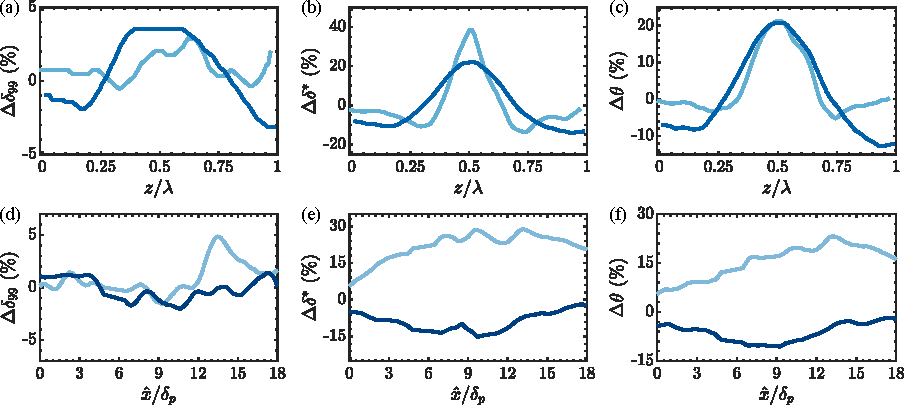
\includegraphics[width = 0.99\textwidth]{figures/results/stereo/TBLstats_xz.pdf}
    \caption{Turbulent-boundary-layer parameters for the strongest actuation case ($V_{pp} = 20 \mathrm{kV}$, $C_\mu = 0.1825$). (a-c) Distribution across the actuator wavelength ($\lambda$) at $\hat{x} = 87\mathrm{mm} \approx 6\delta_p$ \lcap{-}{blue3} and $\hat{x} = 257\mathrm{mm} \approx 18\delta_p$ \lcap{-}{blue5}; (d-e) Evolution along the streamwise direction at $z_1$ \lcap{-}{blue2} and $z_2$\lcap{-}{blue6}.}
    \label{fig:TBLstats_xz}
\end{figure}

%-------
\begin{table}
\centering
\resizebox{\textwidth}{!}{%
%\begin{tabular}{>{\centering}p{0.06\linewidth-2\tabcolsep}
%                >{\centering}p{0.06\linewidth-2\tabcolsep}
%                >{\centering}p{0.11\linewidth-2\tabcolsep}
%                >{\centering}p{0.11\linewidth-2\tabcolsep}
%                >{\centering}p{0.11\linewidth-2\tabcolsep}
%                >{\centering}p{0.11\linewidth-2\tabcolsep}
%                >{\centering}p{0.11\linewidth-2\tabcolsep}
%                >{\centering}p{0.11\linewidth-2\tabcolsep}
%                >{\centering}p{0.11\linewidth-2\tabcolsep}
%                >{\centering\arraybackslash}p{0.11\linewidth-2\tabcolsep}}
\begin{tabular}{llllllllll}
\toprule
$x_{LE}$ & $z$ & $V_{pp}$ & $C_\mu$ & \multicolumn{2}{c}{$\delta$} & \multicolumn{2}{c}{$\delta^*$} & \multicolumn{2}{c}{$\theta$} \\
 &  & $(kV)$ &  & \multicolumn{2}{c}{$(mm)$} & \multicolumn{2}{c}{$(mm)$} & \multicolumn{2}{c}{$(mm)$}\\ \midrule
\multirow{7}{*}{$x_1$} &  & \textbf{0} & \textbf{-} & \textbf{16.1} &  & \textbf{2.66} &  & \textbf{1.82} & \\
 & \multirow{3}{*}{$z_1$} & 10 & 0.0153 & 16.2 & {(+0.3\%)} & 2.75 & \green{(+3.6\%)} & 1.83 & {(+0.5\%)}\\
 &  & 18 & 0.1133 & 16.3 & {(+1.4\%)} & 3.09 & \green{(+16.4\%)} & 1.97 & \green{(+8.5\%)}\\
 &  & 20 & 0.1825 & 16.2 & {(+0.6\%)} & 3.52 & \green{(+32.5\%)} & 2.18 & \green{(+19.7\%)}\\
 & \multirow{3}{*}{$z_2$} & 10 & 0.0153 & 16.0 & {(-0.1\%)} & 2.63 & {(-0.8\%)} & 1.81 & {(-0.6\%)}\\
 &  & 18 & 0.1133 & 16.4 & {(+1.8\%)} & 2.55 & \red{(-3.9\%)} & 1.78 & \red{(-2.3\%)}\\
 &  & 20 & 0.1825 & 16.3 & {(+1.1\%)} & 2.46 & \red{(-7.4\%)} & 1.74 & \red{(-4.5\%)}\\ \midrule
\multirow{7}{*}{$x_2$} &  & \textbf{0} & \textbf{-} & \textbf{18.0} &  & \textbf{2.94} &  & \textbf{2.01} & \\
 & \multirow{3}{*}{$z_1$} & 10 & 0.0153 & 17.7 & {(-1.8\%)} & 2.91 & {(-1.0\%)} & 1.99 & {(-1.0\%)}\\
 &  & 18 & 0.1133 & 18.0 & {(-0.1\%)} & 3.13 & \green{(+6.6\%)} & 2.13 & \green{(+6.3\%)}\\
 &  & 20 & 0.1825 & 18.6 & \green{(+3.3\%)} & 3.47 & \green{(+18.1\%)} & 2.38 & \green{(+18.9\%)}\\
 & \multirow{3}{*}{$z_2$} & 10 & 0.0153 & 18.0 & {(+0.2\%)} & 3.00 & \green{(+2.1\%)} & 2.04 & {(+1.5\%)}\\
 &  & 18 & 0.1133 & 18.1 & {(+0.7\%)} & 2.85 & \red{(-3.2\%)} & 1.95 & \red{(-2.6\%)}\\
 &  & 20 & 0.1825 & 17.9 & {(-0.6\%)} & 2.76 & \red{(-6.0\%)} & 1.91 & \red{(-4.6\%)}\\ \bottomrule
\end{tabular}}
\caption{Experimental parameters of the boundary layers for the cases shown in figure~\ref{fig:UmVmprofile}. The parameters corresponding to the reference TBL are highlighted in \textbf{bold}. Relative change of the experimental parameters with respect to the reference TBL without actuation is between brackets. Positive increments above 2\% are highlighted in \green{green} and negative increments below -2\% in \red{red}.\label{tab:TBLparams}}
\end{table}
%-----

The momentum injection of plasma does not cause any significant modification of $\delta$ along either $x$ or $z$ unlike observations in previous contributions studying streamwise vortices embedded in a TBL \citep{Eibeck1987,Pauley1988,Pauley1994}. Instead, the main contribution of the plasma forcing at $z_1$ is a remarkable increase in the displacement thickness. A larger $\delta^*$ is a direct indication of higher mass flux deficit $\left(\rho\left[ U_\infty-u(y)\right]\right)$ within the boundary layer, which is also seen in the $\overline{U}^+$ profiles shown in figure~\ref{fig:UmVmprofile}(a). Analogously, the increase of momentum thickness is related to a positive increment of the deficit of momentum flux $\left(\rho u(y)\cdot\left[ U_\infty-u(y)\right]\right)$ through the boundary layer. Note, however, that the increment in $\theta$ is less pronounced than the one in $\delta^*$ since the momentum flux deficit is affecting layers where $u$ is small, i.e. in the inner region, thus determining an increase of the shape factor $H$. 

Far downstream from the actuation at $x_2$ ($\hat{x}\approx 16$), the TBL is still reminiscent from the induced vortical motion by the plasma actuator; however, the inner region of the TBL progressively adapts to the new flat-plate, smooth-surface condition, and, hence, the fluid blockage induced by plasma forcing at $z_1$ upstream is considerably reduced as suggested by the $\delta^*$ values. Conversely, the reduction of $\delta^*$ and $\theta$ for $z_2$ is a direct indicator of a reduction in mass- and momentum-flux deficits respectively. 

%%%%%%%%%%%%%%%%%%%%%%%%%%%%%%%%%%%%%%%%%%%%%%%%%% Fluctuations %%%%%%%%%%%%%%%%%%%%%%%%%%%%%%%%%%%%%%%%%%%%
\subsection{Actuation effect on the fluctuating flow field}
The normal streamwise $\overline{u^2}^+$, wall-normal $\overline{v^2}^+$ and premultiplied turbulence production profiles in inner units are reported in figure~\ref{fig:u2v2Pprofile}. Turbulence production is expressed by:
\begin{equation}
    P = -\overline{u_i u_j}\overline{S_{ij}}, \qquad \overline{S_{ij}} = \left( \frac{\partial U_i}{\partial x_j} + \frac{\partial U_j}{\partial x_i} \right),
     \label{eq:TurbProdFull}
\end{equation}
where $u_i$ is the fluctuating $i^{th}$ velocity component, $\overline{S_{ij}}$ is the strain rate tensor and $U_i$ is the $i^{th}$ mean velocity component. %\citep{pope2000}. 
An order-of-magnitude analysis based on stereo-PIV dataset confirms that the dominant component of the turbulence production is $-\overline{uv}\overline{S_{xy}}$. The turbulence production scaled in inner variables $P^+$ can thus be written as
\begin{equation}
    P^+ \approx -\overline{uv}^+ \frac{\partial U^+}{\partial y^+}. \label{eq:TurbProdRed}
\end{equation} 
%
\begin{figure} % TBL profiles
    \centering
    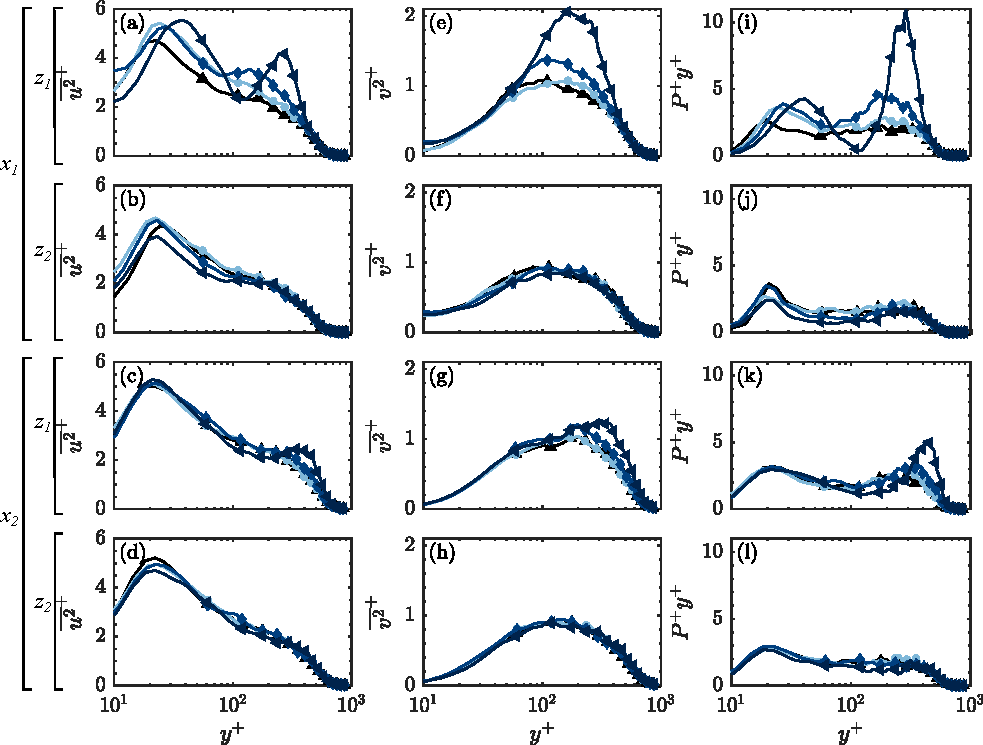
\includegraphics[width = 0.99\textwidth]{figures/results/TBL/u2_v2_P_profilesv2}
        \caption{Inner-scaled fluctuating velocities at selected stations according to figure~\ref{fig:setup}. $\overline{u^2}^+$, $\overline{v^2}^+$ and $P^+y^+$ profiles are depicted in the left column (a-d), center column (e-h) and right column (i-l) respectively, for selected discharge voltages $V_{pp}=$ (and momentum coefficient $C_\mu = $) 0 \sy{black}{t*}, 10 (0.0153) \sy{blue2}{o*}, 18 (0.1133) \sy{blue6}{d*}, 20 (0.1825) \sy{blue7}{lt*}.}
    \label{fig:u2v2Pprofile}
\end{figure}%
Focusing on the spanwise station $z_1$, there is a clear effect of the induced jets on the position and intensity of the inner peak of $\overline{u^2}^+$, and on the turbulent fluctuations in the outer layer. The inner peak is displaced away from the wall, while an outer peak is produced at the outer layer. The latter effect becomes evident for increased forcing. Moreover, the $\overline{u^2}^+$ profile exhibits a valley between both peaks, which becomes more pronounced with increasing amplitude of actuation. An outer peak is also observed in the profile of $\overline{v^2}^+$. The shape of the profiles depicted in figure~\ref{fig:u2v2Pprofile}(a) is likely due to enhanced large-scale motions.
The displacement of the inner peak in $\overline{u^2}^+$ can be ascribed to the mutual interaction between wall-tangent plasma jets which are lifted away from the wall as the forcing becomes stronger. The outer peak in $\overline{u^2}^+$ corresponds to the wall-normal location of the onset of the streamwise vortices. This is in accordance with the pronounced reduction between the inner and the outer peak, where there is a considerable component of wall-normal velocity induced by the vortex interaction as described for the mean-fields in figure~\ref{fig:UmVmprofile}(e). Moreover, the profiles of $\overline{v^2}^+$ show a peak that coincides with the valley in $\overline{u^2}^+$, at the region where the pair of counter-rotating vortices couple to promote a wall-normal motion. The values of $\overline{u^2}^+$, $\overline{v^2}^+$ at $z_2$ are almost unaltered with respect to the reference TBL as shown in figure~\ref{fig:u2v2Pprofile}. Therefore, plasma forcing is mainly affecting the mean-field in the vicinity of $z_2$ while it is very effective in manipulating both fluctuating and mean-field for the plasma side where the opposing plasma jets collide and generate wall-normal motion $(z_1)$. Focusing on the downstream persistence of the actuation, figure~\ref{fig:u2v2Pprofile}(c,g) show how both $\overline{u^2}^+$ and $\overline{v^2}^+$ rapidly adjust to the new wall condition without actuation within the wall region. On the other hand, the perturbation of the outer layer is more persistent, as presented in the form of a localised increase in $\overline{u^2}^+$ and $\overline{v^2}^+$ at $y^+\approx 400$ and $y^+\approx 300$ respectively.

The inner-scaled turbulence production in the premultiplied form $P^+y^+$ (calculated from equation~\ref{eq:TurbProdRed}) is preferred since, when represented in semi-logarithmic form, equal areas correspond to equal contributions to the production \citep{Marusic2010wbt}. ZPG TBLs are characterised by a relatively flat $P^+y^+$ distribution as shown for $V_{pp} = 0 kV$ case in figure~\ref{fig:u2v2Pprofile}(i-l). In the case of plasma actuation, the effect at $z_1$ presents some analogies with that observed in APG TBLs, with a production peak in the outer layer \citep{harun2013pressure,bradshaw1967}. Interestingly, the position of the production peak at $z_1$ coincides with the peak in the $\overline{uv}$, meaning that the main effect of the plasma actuation is to change the distribution of energy through the boundary layer, displacing large energetic structures from the near-wall region to the outer region. Although the DBD-actuator increases $\delta^*$ and $\theta$, and forces the flow in the wall-normal direction, the value of $\delta$ is almost unaffected. Hence, as the effect of the actuation is displaced downstream and for the strongest forcing, the production peak is shifted toward higher $y^+$. In contrast, at the spanwise station $z_2$, the effect on $P^+y^+$ exhibits a distribution that resembles that of a ZPG-TBL or even an FPG-TBL. However, for the streamwise station closer to the actuator ($x_1$), the plasma-induced jets seem to effectively reduce the turbulence production within the logarithmic layer with respect to the non-actuated case. Such an opposite phenomenon is in accordance with the reduction of displacement and momentum thickness of the TBL and the suction motion induced by the discharge, which eventually displaces the fluid in the logarithmic and outer region of the TBL towards the wall.

It becomes evident that the plasma induces spanwise and wall-normal motions in the near-wall layer. The peak in $\overline{v^2}^+$ occurs at $y^+= 110$, whilst $P^+y^+$ has two peaks, occurring at $y^+ = 40$ and $y^+ = 120$. One can interpret these mean locations as the bottom, centre, and top of the plasma-induced streamwise vortices. The peak in $\overline{v^2}^+$ closely corresponds to the position of the average height of the plasma-induced streamwise vortex cores due to the low momentum fluid entrained within them, and due to wall-normal induced vortex motions to either side of the core. The first peak of $P^+y^+$ marks the lower extent of the plasma vortices due to spanwise induced vortex motions below the core, and also corresponds to the location of the maximum $\overline{u^2}^+$. The second peak of $P^+y^+$ corresponds to the upper extent of the vortices and also coincides with the location of the second $\overline{u^2}^+$ peak. 

A final comment can be made on the phenomena described by the turbulence intensity downstream of the actuation. In figures~\ref{fig:u2v2Pprofile}(k,l), it is observed that the smaller energetic scales in the buffer region are already adjusted to the new wall condition. Conversely, the large-scale motions, which are over-energised (relative to the new smooth-wall boundary condition), retain a strong footprint within the boundary layer, extending deep into the buffer region. Similar results were achieved by \citet{jukes2006TBLcontrol} with a 40\% reduction in mean streamwise velocity and a 30\% reduction in turbulent intensity observed for $y^+< 30$.

%%%%%%%%%%%%%%%%%%%%%%%%%%%%%%%%%%%%%%%%%%%%%%%%%%%%%%%%%%%%%%%%%%%%%%%%%%%%%%
%%%%%%%%%%%%%%%%%%%%%%%%% Stanton number measurements %%%%%%%%%%%%%%%%%%%%%%%%
%%%%%%%%%%%%%%%%%%%%%%%%%%%%%%%%%%%%%%%%%%%%%%%%%%%%%%%%%%%%%%%%%%%%%%%%%%%%%%
\section{Wall distribution of the Stanton number}\label{s:resultsSF}
%---
\begin{figure}[h]
         \centering
         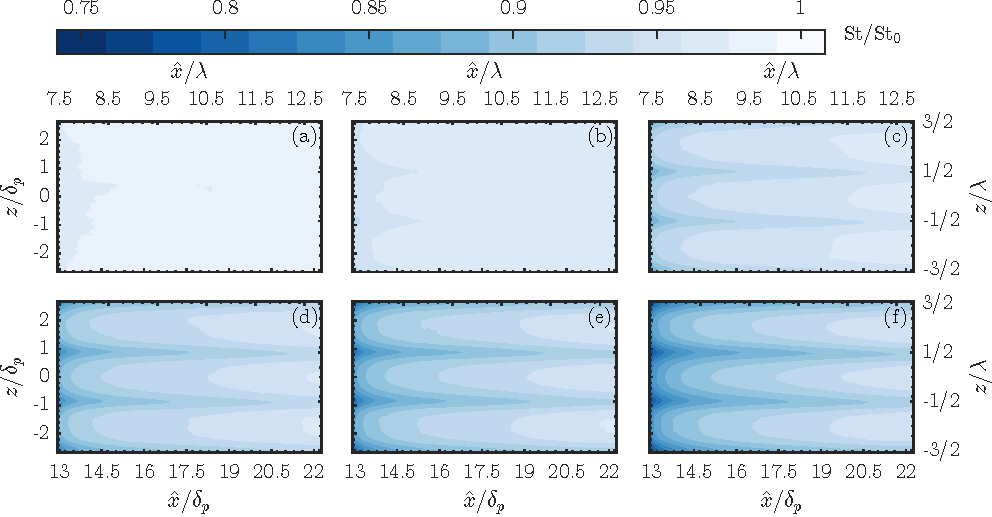
\includegraphics[width=0.99\linewidth]{figures/results/St/st_rebut.pdf}
         \caption{$\mathrm{St}(x,z)/\mathrm{St_0}(x,z)$ distribution on the region of interest for the tested discharge voltages $V_{pp}=$  (and momentum coefficient $C_\mu = $) 10 (0.0153) (a), 12 (0.0278) (b), 14 (0.0484) (c), 16 (0.0711) (d), 18 (0.1133) (e), 20 (0.1825) (f).} \label{fig:st_maps} % [0 0.0153,0.0278,0.0484,0.0711,0.1133,0.1825]
\end{figure}
%---
Infrared thermography measurements with a PCB as a heat-flux sensor are carried out to understand whether the persistent perturbation in the outer layer by the plasma actuation has a corresponding footprint on the convective heat transfer at the wall. Based on the conclusion that the plasma momentum injection, perpendicular to the main stream, triggers the formation of pairs of counter-rotating vortices, the calculation of the Stanton number at the wall aims at corroborating the behaviour of such large-scale motion and its persistence in the far-field downstream of the actuation. 
The time-averaged Stanton number distributions on the wall downstream of the control region for the different plasma discharge voltages are shown in figure~\ref{fig:st_maps}. The results are normalised with the wall-distribution of Stanton number at non-actuated flow conditions $\mathrm{St}_0$. A region of interest is considered, covering two pairs of DBD-actuators in the spanwise direction (approximately 1.5$\lambda$ at each side of the symmetric, $xy$-plane) and a considerable range in the streamwise direction of $13\leq\hat{x}/\delta_p\leq 22.5$. Note that the IR images are taken at a distance of 13$\delta$ from $x_p$, which implies a physical distance of $185\mathrm{mm}$ from the upstream edge of the plasma discharge and $55\mathrm{mm}$ from its downstream edge.  

Analysing the weakest plasma forcing configuration in figure~\ref{fig:st_maps}(a), it is clear that the actuation tends to uniformly reduce the Stanton number for the whole region of interest. As the discharge voltage is increased, a localised, more significant $\mathrm{St}$ reduction is evident at the location where plasma jets oppose each other. Therefore, the plasma forcing is composed of two main effects on the Stanton number distribution: a uniform reduction, and a localised decrease at the location where the plasma-induced jets lift-off. The first contribution can be understood as a consequence of the increased momentum defect in the inner region, which thus results in reduced heat transfer. On the contrary, the second effect promotes the streak-like pattern identified at $z/\lambda \approx \pm 1/2$. The superposition of both contributions becomes evident when computing the normalised, streamwise average over the region of interest $\langle \mathrm{St} \rangle$, shown in figure~\ref{fig:meanSt_delta}(a),
\begin{equation}
    	\langle \mathrm{St} \rangle = \int \mathrm{St}(x,z) \,\mathrm{d}x .
\end{equation}
The uniform reduction in convective heat transfer at the wall grows with the intensity of the actuation, corroborating the monotonic increase in actuation effectiveness with $C_\mu$ as previously reported from the TBL profiles. Similarly, the irregular actuation generating the streak-like pattern also intensifies, causing higher amplitudes in the oscillation along with the spanwise component.  
%----
\begin{figure}
         \centering
         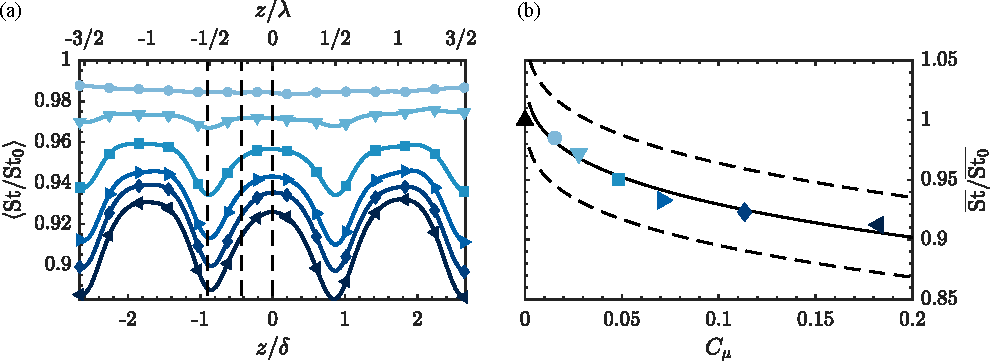
\includegraphics[width=0.99\linewidth]{figures/results/St/stz_v3_cmu.pdf}
         \caption{(a) Streamwise average of Stanton number in the region of interest shown in figure~\ref{fig:st_maps} normalised with the reference TBL; reference lines \lcap{--}{black} highlight $z_1$, $z_2$ and plane of symmetry spanwise stations from left to right. (b) Spatial average of the Stanton number in the region of interest as a function of the body force with the fit for the empirical relation $\overline{\mathrm{St}} \propto C_\mu ^{2/7} $ \lcap{-}{black} and $\pm3.7\%$ error interval \lcap{--}{black}. Symbols correspond to each discharge voltages $V_{pp}=$ (and momentum coefficient $C_\mu = $) 0 \sy{black}{t*}, 10 (0.0153) \sy{blue2}{o*}, 12 (0.0278) \sy{blue3}{dt*}, 14 (0.0484) \sy{blue4}{s*}, 16 (0.0711) \sy{blue5}{rt*}, 18 (0.1133)
         \sy{blue6}{d*}, 20 (0.1825) \sy{blue7}{lt*}.} \label{fig:meanSt_delta}
\end{figure}
%---

The uniform distribution of $\mathrm{St}$ measured for the weakest actuation suggests that the large-sale motion introduced at the control region is not sufficiently strong to persist downstream and rapidly diminishes. Nonetheless, the heat transfer reduction at the wall persists even after the dissipation of the plasma-induced flow, which was reported by \citet{Schoppa1998} for a spanwise control law in channel flows and recently concluded in \citet{cheng_wong_hussain_schroder_zhou_2021} for similar plasma-actuators vortex generators in TBLs. The large structures collapse just downstream of the DBD-actuator, diffusing into lower scales that uniformly distribute within the boundary layer, thus promoting a homogeneous reduction in heat transfer. As the forcing amplitude is increased, so is the intensity of the large-scale structures which are able to persist in space and time as can be assessed from their thermal footprint. The conclusions drawn from the IR thermography analysis confirm the proposed explanation exposed in \S\ref{s:TBLanalysis}, justifying the formation of pairs of counter-rotating vortices. 

Upon the activation of plasma discharge, a downwash occurs between electrodes (plasma side), as the plasma actuator entrains fluid from above, ejecting it laterally. It has been shown that the plasma causes a large streamwise velocity deficit in the buffer and logarithmic region of the boundary layer that is persistent downstream. This deficit is related to the formation of streamwise vortices, which also alters the near-wall velocity gradient, thus reducing turbulent fluxes as is the case of convective heat transfer at the wall. The plasma-induced vortices superpose their upwash/downwash from adjacent vortices, causing increased transport of high-momentum fluid towards the wall by vortex induction, and conversely, pushing more low-momentum fluid from the near-wall region away from the surface. This approach is very similar to that proposed by \citet{jukes2013plasmaVG}, in which the combination of two elongated electrodes in the direction of the flow leads to what they defined as \textit{DBD-plasma actuator vortex generator}, which was also exploited in turbulent boundary layers as for the case of \citet{Wicks2015}.
The mutual induction between vortex pairs at $z_1$ displaces the fluid from the lower region of the boundary layer to the outer region, extracting low-speed fluid with high turbulent intensity from the wall, locally minimising heat transfer. On the other hand, streamwise vortices are weaker at $z_2$. The plasma-induced suction enables the formation of the vortex, which locally enhances the mixing between the outer and lower regions of the TBL. 
 
The study by \citet{cheng_wong_hussain_schroder_zhou_2021} concludes that the local reduction in skin friction is due to the reorganisation of the TBL streaks within the turbulent boundary layer. The ‘artificial’ vortices introduced by the plasma actuation and their associated spanwise wall jets act as a mechanism of merging natural streaks. Furthermore, their flow visualisation results show that the resultant streak is wider and has reduced meandering in space. This wider streak resembles the low-speed ribbon centred at $z_1$ in the present study. \citet{cheng_wong_hussain_schroder_zhou_2021} attribute the effect of forcing as a stabilisation of the streak-alike structure, thus interrupting the turbulence regeneration cycle and reducing the production of turbulent fluxes. This conclusion is also supported by the TBL analysis performed in the present study. The streamwise velocity is locally reduced in the region where ejection occurs while it is increased at both sides due to the spanwise diversion of the flow. Such velocity and momentum flux deficit incurred by the plasma forcing are persistent in space and time as extracted from the values of $\delta^*$ and $\theta$ reported in table~\ref{tab:TBLparams}. Consequently, the local heat transfer at the wall is modified according to the local flow condition at the wall.

Figure~\ref{fig:meanSt_delta}(b) depicts the evolution of the spatially averaged Stanton number, defined as:
\begin{equation}
    	\overline{\mathrm{St}} = \iint {\mathrm{St}(x,z)} \,\mathrm{d}x\,\mathrm{d}z.
\end{equation}
Considering that the weakest actuation ($C_\mu = 0.015$, i.e. $V_{pp}=10\mathrm{kV}$) hereby reported is found to be the threshold value for generating a plasma discharge, the results show that the value of $\overline{\mathrm{St}}$ follows a linear relation with the discharge voltage. Recalling that the integrated body force in non-dimensional form, i.e. the momentum coefficient $C_\mu$, scales with the discharge voltage to the $7/2$ power as reported in figure~\ref{fig:plasma_char}, a proportional relation can be expressed between the spatially-averaged Stanton number and the momentum coefficient: $\overline{\mathrm{St}} \propto C_\mu^{2/7}$. This relation reasonably matches the experimental data as shown in figure~\ref{fig:meanSt_delta}(b), with the Stanton number being reduced with the momentum injection promoted by plasma. Eventually, the plasma forcing provides a reduction of 9\% in convective heat transfer for the strongest actuation, which reaches values of 11\% reduction along with the streaks (see figure \ref{fig:meanSt_delta}), in close agreement with the skin-friction drag reduction of 7\% reported in \citet{cheng_wong_hussain_schroder_zhou_2021}. 

The proposed actuation, characterised by a jet spacing of $\Delta z^+ \approx 450 ~(=\lambda^+/2)$ and an intensity of $8\%$ of the free stream velocity, resembles to the proof-of-principle test proposed by \citet{Schoppa1998} for drag reduction. They reported a significant sustained drag reduction of 20\% which they attested to the weakened longitudinal vortices near the wall due to forcing-induced suppression of an underlying streak instability mechanism. The production of wide ribbons of low-speed streamwise velocity take a relevant part in the drag reduction mechanism. This approach to reducing turbulent wall fluxes is common in studies that employ spanwise travelling waves \citep{Du2002, Whalley2014} or spanwise wall-jet forcing \citep{yao2017,yao2018}. These studies, although using a different control strategy, achieve similar results in terms of wall-fluxes reduction by the generation of mutually interacting streamwise vortices. Indeed, the alteration of the near-wall flow, transforming sublayer streaks into wide ribbons of low-speed fluid is a relevant and persistent conclusion in the present study.

%%%%%%%%%%%%%%%%%%%%%%%%%%%%%%%%%%%%%%%%%%%%%%%%%%%%%%%%%%%%%%%%%%%%%%%%%%%%%%
%%%%%%%%%%%%%%%%%%%%%%%%%%%%%%% CONCLUSIONS %%%%%%%%%%%%%%%%%%%%%%%%%%%%%%%%%%
%%%%%%%%%%%%%%%%%%%%%%%%%%%%%%%%%%%%%%%%%%%%%%%%%%%%%%%%%%%%%%%%%%%%%%%%%%%%%%%
\section{Conclusions} \label{s:conclusions}
The utilisation of plasma actuators as vortex generators to control convective heat transfer in a turbulent boundary layer is investigated experimentally. In particular, an array of plasma actuators is used to induce pairs of counter-rotating, stationary, streamwise vortices embedded in a turbulent boundary later. The analysis focuses on the mechanism of interaction between the plasma-induced large-scale structures and the convective heat transfer process in a fully developed turbulent boundary layer over a flat plate with ZPG conditions. The combination of flow-field and heat-transfer measurements allows to understand the physics behind the plasma-induced flow.

A convective heat transfer reduction mechanism is proposed. The current plasma control technique focuses on manipulating near-wall coherent structures, which are responsible for turbulent transport phenomena within the TBL. Large-scale pairs of counter-rotating streamwise vortices are generated upon the activation of the plasma discharge. The proposed DBD-plasma actuator array is shown to be robust, with long-life applicability without loss of effectiveness.

The generation of pairs of counter-rotating, streamwise vortices is confirmed by the reconstructed three-dimensional mean flow field. Upon the activation of plasma, the fluid ejected laterally by the discharge is replenished by entertainment from above the exposed electrodes. This generates a circulation in the lateral plane leading to a vortical motion. The coalescence of the plasma-induced circulation with the main stream leads to twisting and folding of the spanwise vorticity at the tip of each plasma actuator. Eventually, wall-normal mean vorticity is produced by the body force, which reorients into the streamwise direction, while the spanwise mean vorticity is also reoriented into the streamwise direction. These phenomena have been previously reported by \citet{jukes2013plasmaVG} for a single actuator aligned with the main flow and by \citet{Wicks2015} for an array similar to the one proposed here. Additionally, the induced streamwise vortices are confirmed to be stationary according to the persistence theory of turbulence \citep{Cotel1996stationary}. The suction promoted over the exposed electrodes of the plasma-actuator array locally confines the vortices, preventing them to expand in the spanwise direction. The stationary vortices reduce wall fluxes as demonstrated for the convective heat transfer wall distribution downstream. 

Furthermore, an in-depth analysis of the turbulent boundary layer and its statistical parameters is performed. The plasma-induced flow diverts the TBL within the inner region, close to the wall and two main effects are outlined: on one hand, at the location where the wall-tangent opposing plasma-induced jets collide (namely, $z_1$), a mass and momentum flux deficit is observed due to a considerable reduction of the streamwise velocity component by the upwelling motion induced by the plasma; and, on the other hand, over the exposed electrodes (namely, $z_2$), a moderate reduction of mass and momentum flux deficit is detected as a consequence of the flow diversion and subsequent acceleration. The former effect causes a considerable increase of $\delta^*$ and $\theta$ with respect to the non-actuated TBL while the latter yields the opposite result.

These conclusions are in agreement with the recent contribution by \citet{cheng_wong_hussain_schroder_zhou_2021}, albeit conducted here at significantly larger freestream velocity and momentum injection. The wall-tangent injection of momentum by plasma forces the TBL streaks together, which eventually merge and stabilise. A wide ribbon of low-speed fluid is promoted and stabilised by plasma actuation at $z_1$. The generation of wide ribbons of low-speed fluid is a common strategy as a drag reduction mechanism \cite[e.g.][]{Schoppa1998,Du2002, Whalley2014,cheng_wong_hussain_schroder_zhou_2021} and, analogously, it is concluded that it is a strategy that is also efficient for reducing heat fluxes at the wall.

Considering the IR thermography analysis, it is concluded that the plasma-induced flow is persistent downstream, with remarkable consequences on the heat transfer distribution. Wide ribbons of Stanton number reductions are observed at $z_1$, suggesting that the velocity deficit promoted by plasma endures downstream of the actuation with an effective reduction of wall fluxes. Despite the spanwise modulated Stanton number distribution, a consistent reduction of spatially integrated heat transfer is observed for increasing intensity of the forcing amplitude. Eventually, it is concluded that the Stanton number over an actuator pitch scales linearly with the discharge voltage, i.e. with the $2/7$ power of the momentum coefficient $C_\mu$. This interesting result summarises with an overall reduction of $\approx10\%$ of the Stanton number far downstream of the actuation and for a wide region of interest. 

%%%%%%%%%%%%%%%%%%%%%%%%%%%%%%%%%%%%%%%%%%%%%%%%%%%%%%%%%%%%%%%%%%%%%%%%%%%%%%%
%%%%%%%%%%%%%%%%%%%%%%%%%% Acknowledgements %%%%%%%%%%%%%%%%%%%%%%%%%%%%%%%%%%%
%%%%%%%%%%%%%%%%%%%%%%%%%%%%%%%%%%%%%%%%%%%%%%%%%%%%%%%%%%%%%%%%%%%%%%%%%%%%%%%

\section*{Acknowledgements}
Rodrigo Castellanos, Stefano Discetti and Andrea Ianiro have been supported by the project ARTURO, ref. PID2019-109717RB-I00/AEI/10.13039/501100011033, funded by the Spanish State Research Agency.
Theodoros Michelis and Marios Kotsonis are supported by the European Research Council under StG project GloWing (\#803082).

\section*{Declaration of Interest}
The authors report no conflict of interest.